\documentclass[11pt,openright,twoside]{book}
\usepackage[a5paper,bottom=2.3cm,top=2.3cm,inner=1.3cm,outer=1.8cm,headheight=14pt]{geometry}
%\usepackage[width=158.5mm, height=220mm,center,cam,noinfo]{crop}

\usepackage[italian]{babel}
\usepackage[utf8]{inputenc}
\usepackage[T1]{fontenc}

\usepackage{textcomp}
\usepackage{graphicx} % per immagini
\usepackage{fancyhdr}%per intestazione personalizzata
\usepackage[bookmarks,hidelinks]{hyperref} % for pdf index and links
\usepackage{booktabs}
\usepackage{tabularx}
\usepackage{cite} % for citation grouping
\usepackage{pdfpages}
%\usepackage[autostyle]{csquotes}
\usepackage{multirow}
\usepackage{tabularx}
\usepackage{ltablex}
\usepackage{bigstrut}
\usepackage{needspace}
\usepackage{emptypage}
\usepackage{wrapfig}
\usepackage{rotating}
\usepackage[font=small,skip=15pt]{caption}

%%========================================================
%%     modifica dimensioni e formato del titolo dei capitoli
%%
\usepackage{titlesec,color}
\newcommand{\hsp}{\hspace{10pt}}
\titleformat{\chapter}[hang]{\LARGE\bfseries}{\thechapter\hsp}{0pt}{\LARGE\bfseries}
\titlespacing*{\chapter}{0cm}{-\topskip+20pt}{20pt}[0pt]
%%
%%========================================================

\newenvironment{italico}{\itshape}

%%========================================================
%%     modifica toc
%%
\usepackage[titles]{tocloft}
\renewcommand{\cftdotsep}{0}
\renewcommand{\cftchapfont}{\normalfont\normalsize}
\renewcommand{\cftchappagefont}{\normalfont\normalsize}
\renewcommand{\cftchapleader}{\cftdotfill{\cftsecdotsep}}
%\renewcommand\cftchapafterpnum{\vskip0pt}
\setlength{\cftbeforesecskip}{10pt}
\setlength{\cftbeforesubsecskip}{5pt}
%\renewcommand\cftsecafterpnum{\vskip10pt}
%%
%%========================================================

%%========================================================
%%     carattere
%%
\usepackage{lmodern} % Latin modern
\usepackage[sc]{mathpazo} % Palatino
\linespread{1.05}
%\usepackage{kpfonts} %Palatino
%\usepackage{mathptmx} %Times
%%
%%========================================================

%\setlength{\parindent}{0cm} %Disabilita indentazione dei paragrafi
\renewcommand{\arraystretch}{1.4} % per le tabelle
\renewcommand{\labelitemi}{--} % per gli elenci puntati
\def\tabularxcolumn#1{m{#1}} %centra verticalmente
\newcolumntype{s}{>{\centering\arraybackslash\hsize=.5\hsize}X} %centra orizzontalmente

%%========================================================
%%     Permette di inserire un pdf come immagini
%%
\makeatletter
\newcounter{imagepage}
\newcommand*{\foreachpage}[2]{%
  \begingroup
    \sbox0{\includegraphics{#1}}%
    \xdef\foreachpage@num{\the\pdflastximagepages}%
  \endgroup
  \setcounter{imagepage}{0}%
  \@whilenum\value{imagepage}<\foreachpage@num\do{%
    \stepcounter{imagepage}%
    #2\relax
  }%
}
\makeatother
%%
%%========================================================

%%========================================================
%%     previene l'interruzione di pagina su tabelle lunghe in caso di utilizzo multirow
%%
\makeatletter
\def\@cline#1-#2\@nil{%
  \omit
  \@multicnt#1%
  \advance\@multispan\m@ne
  \ifnum\@multicnt=\@ne\@firstofone{&\omit}\fi
  \@multicnt#2%
  \advance\@multicnt-#1%
  \advance\@multispan\@ne
  \leaders\hrule\@height\arrayrulewidth\hfill
  \cr
  \noalign{\nobreak\vskip-\arrayrulewidth}}
\makeatother
%%
%%========================================================

%%========================================================
%%            personalizzazione intestazione
%%
\pagestyle{fancy}
\renewcommand{\chaptermark}[1]{\markboth{#1}{}}
\renewcommand{\sectionmark}[1]{\markright{\thesection\ #1}}
\fancyhf{}
\fancyfoot[C]{\thepage}
\fancyhead[CE]{\nouppercase\leftmark}%\nouppercase elimina tutte le intestazioni maiuscole
\fancyhead[CO]{\nouppercase\rightmark}%\nouppercase elimina tutte le intestazioni maiuscole
\renewcommand{\headrulewidth}{0pt}
\renewcommand{\footrulewidth}{0pt}
%%
%%========================================================

\newcommand*\cleartoleftpage{%
  \clearpage
	\thispagestyle{empty}
  \ifodd\value{page}\hbox{}\newpage\fi
}

%%========================================================
%%   per imporre sillabazione
%%
\hyphenation{Enzo Marisa Pianigiani Federico}%
%%========================================================

\begin{document}
\raggedbottom % Prevent vertical justification

%=========================================
\begin{titlepage}
        \vspace*{10mm}
		\centering{
			\Large{\sffamily PARROCCHIA di SAN FRANCESCO in TRIESTE\par }\bigskip{\fontsize{22}{22}\selectfont\bfseries 1965-2015: 50 ANNI di VITA\par }\bigskip LA COMUNITÀ RACCONTA\par
		}
			
		\vspace{10mm}
		\vspace{\fill}
		\centering \large{Trieste 2015}
\end{titlepage}

%=========================================
\thispagestyle{empty}
\vspace*{15ex}
\begin{flushright}
\textit{Altissimu, onnipotente, bon Signore,\\
tue so’ le laude, la gloria e \\
l’honore et onne benedictione.\\}
\vspace{2ex}
\scriptsize{San Francesco d'Assisi}
\end{flushright}
\cleardoublepage

\chapter*{Presentazione}
\label{chap:abstract}
\addcontentsline{toc}{chapter}{Presentazione}
E’ davvero un onore, per me, presentarvi questo opuscoletto in memoria e celebrazione dei
50 anni della nostra bella parrocchia di s. Francesco. Nella riunione del Consiglio Parrocchiale 
abbiamo raccolto alcune idee per celebrare e ricordare questo avvenimento, che cade giusto nella 
festa del nostro Patrono. E perché non riportare anche per iscritto i momenti salienti della crescita 
(strutturale, pastorale e spirituale) di una comunità di cristiani? E così è nato questo libricino, con 
l’unico intento di raccontare il cammino della comunità di san Francesco, attraverso i suoi 
protagonisti ancora viventi: pastori e fedeli.
\begin{center}
	\textbf{3 OTTOBRE 1965 – 4 OTTOBRE 2015: 50 anni di storia.}
\end{center}

Qualcuno aggiungerebbe: “Di acqua sotto i ponti ne è passata tanta!”. E lo direbbe con molta 
ragione. Davvero la comunità di san Francesco in Trieste deve ringraziare tanto il Signore, e 
continuare a lodarlo e invocarlo perché non venga mai a mancare una sapiente guida (Vescovi e 
frati), una fede pura ed umile, una carità ardente, una gioiosa speranza ed un popolo fedele ed unito. 
\bigbreak

Il libretto che avete per le mani è lungi dall’essere una descrizione esaustiva ed ordinata di 
quanto è avvenuto nel territorio e nel cuore della gente: dovrete aspettare qualche altro buon 
parroco più dotato, paziente e libero del sottoscritto.
Qui ci limitiamo a presentarvi: la “Lettera fondazionale” della parrocchia, con la convenzione tra la 
Diocesi di Trieste e la Provincia religiosa dei Frati Minori Conventuali; l’augurio del Vescovo 
Santin; la Planimetria, con l’elenco aggiornato delle vie e dei numeri civici appartenenti alla 
parrocchia (sostanzialmente tolti dalla parrocchia di san Giovanni Decollato); il racconto dei parroci  
ancora viventi, delle suore Dimesse e quello di due gruppi di parrocchiani, dividendo il periodo in 
due parti (1967-1990; 1990-2015).
 
A lode e gloria di Dio!
\begin{flushright}
	\textit{fra Tiberio Zilio}
\end{flushright}
\chapter*{Saluto dell’Arcivescovo\\ di Trieste}
\addcontentsline{toc}{chapter}{Saluto dell’Arcivescovo di Trieste}
Il 3 ottobre 1965, il mio amato predecessore S. E. Mons. Antonio Santin, con un decreto  
fondazionale, provvedeva ad erigere, nella Diocesi di Trieste, la parrocchia dedicata a San 
Francesco, affidandola alla cura pastorale dei Frati Conventuali. Il ricordo di quella data è motivo di 
gioiosa riconoscenza al Signore per tutte le grazie che, fino ad oggi, ha riservato alla comunità 
parrocchiale e a tutta la Chiesa di Trieste. La grazia del servizio generoso di tanti padri francescani 
che hanno speso le energie migliori del loro ministero per annunciare il Vangelo e per testimoniare 
la carità verso i poveri; la grazia di tantissimi bambini e bambine, di giovani che in parrocchia 
hanno imparato ad amare Dio e ad essere cittadini esemplari; la grazia di tante famiglie che nella 
comunità hanno rafforzato il loro amore e affrontato tante difficoltà; la grazia di tanti poveri, di 
tante persone sole e anziane, che nei fratelli e nelle sorelle della comunità di  san Francesco  hanno 
trovato consolazione e sostegno; la grazia di tanti collaboratori pastorali – catechisti, volontari, 
operatori della caritas… - che, nell’arco di questi cinquant’anni, hanno impreziosito la comunità 
con la testimonianza genuina delle loro opere buone; la grazia della Parola - quella di Gesù e quella 
che è Gesù - che ha convertito e rigenerato innumerevoli anime; la grazia dei sacramenti, soprattutto 
quelli dell’Eucaristia, del Battesimo e della Confessione che sono stati il nutrimento indispensabile 
per dare vita e identità autentiche alla comunità cristiana; la grazia della preghiera e quella della 
vocazione alla santità che Dio rivolge a tutti.
Cinquant’anni di vita cristiana vissuta insieme sotto la protezione di San Francesco; 
cinquant’anni che hanno registrato il miracolo quotidiano dell’amore misericordioso di Dio. Ora, 
doverosamente, la memoria deve aprire i cuori e le menti al futuro affinché la comunità si 
predisponga a viverlo - nella fede, nella speranza e nella carità cristiane - con la stessa fedeltà e il 
medesimo entusiasmo.
Nell’affidare la parrocchia di San Francesco alla materna protezione di Maria, Madre della 
Chiesa, colgo l’occasione per benedire tutti e di cuore.
\begin{flushright}
+Giampaolo Crepaldi\par
Arcivescovo – Vescovo di Trieste
\end{flushright}

\chapter*{Augurio del Ministro Provinciale\\ OFM Conv.}
\addcontentsline{toc}{chapter}{Augurio del Ministro Provinciale OFM Conv.}
\begin{center}
\bfseries
	Per i 50 anni della nostra Parrocchia\par San Francesco in Trieste
\end{center}
``Ti adoriamo, Signore nostro Gesù Cristo, qui e anche in tutte le chiese che sono nel mondo 
intero e ti benediciamo, perché con la tua santa croce hai redento il mondo” (Fonti francescane 
111). Mi affiora alla mente questa preghiera del Serafico Padre nella lieta ricorrenza dei 50 anni 
della Parrocchia di Trieste intitolata proprio a lui ed affidata dalla Diocesi all’animazione della 
nostra Provincia religiosa di Frati Minori Conventuali. È una preghiera che Francesco trovò ed 
elaborò sino a farla sua per poi consegnarla ai suoi frati e a quanti incontrava; un testo che gli 
faceva sobbalzare il cuore. Se ne intendeva di chiese il giovane Francesco: era nata tra queste, fra le 
più derelitte, la sua vocazione, giù nella piana di Assisi, ai margini della città, tra chiese 
abbandonate e corpi trascurati di lebbrosi. Entrambe queste realtà lo videro “restauratore” con 
mattoni e con lo sguardo, la vicinanza fattiva di chi dà dignità a chi l’aveva smarrita. Ognuna di 
queste “due” chiese, quella cadente di San Damiano e quella sofferente dei fratelli lebbrosi, aveva 
bisogno l’una dell’altra e rimandava al proprio tesoro: il Signore Gesù presente nella chiesa di 
mattoni e nei fratelli poveri, messi ai margini, scartati dai più. Iniziò così l’avventura che potremmo 
definire ``parrocchiale'' di Francesco che sino a quel momento della sua vita, si era concentrato 
unicamente su di sé, sui suoi sogni di autorealizzazione. Parafrasando un po' un testo noto: ``Dolce è 
sentire - è la scoperta di Francesco! - che non sono più solo, ma che son parte di una immensa vita, 
di una comunità di fratelli e sorelle, dono del Signore, del suo infinito amore…''
\bigbreak
``Francesco, va’, ripara la mia casa che, come vedi, è tutta in rovina'' (Fonti Francescane 
593). Cominciò così, con l’adesione semplice ed immediata all’invito del Crocifisso di San 
Damiano che gli aveva parlato trafiggendo di dolcezza il suo cuore, la vocazione di Francesco. 
Anche come manovale e muratore. Da allora, sino alla piena “conformitas”- conformità con il 
Crocifisso nel segno delle stigmate sul monte della Verna, quasi al finire dei suoi giorni, l’amore 
per il suo Signore fattosi uomo per noi, fu il centro del cuore di frate Francesco, dei suoi affetti, 
della sua predicazione. Meditava sempre, dice il suo primo biografo, fra Tommaso da Celano, 
“l’umiltà dell’incarnazione e la carità della passione” di Gesù, sino a piangere di commozione e di 
sofferenza quando constatava che “l’Amore non è amato”. Volle assomigliargli in tutto: con l’abito 
di sacco fatto a forma di croce, scegliendo il segno del Tau che riproduce la croce e, soprattutto, 
volendo per sé e i suoi frati una via di povertà e condivisione da vivere in letizia.

Fu solo più avanti che frate Francesco comprese che l’invito a “riparare la chiesa”
riguardava non solo gli edifici cadenti, ma l’edificio vivente della Chiesa. A dirla tutta, quella  del 
suo tempo era una Chiesa non molto edificante, anzi, bisognosa  di riforma, di un ritorno autentico 
al Vangelo, alla sua freschezza. Le chiese “poverelle” ed abbandonate incontrate da Francesco fuori 
Assisi erano come lo specchio della decadenza della Chiesa che attendeva  una vera e propria 
rifondazione. Frate Francesco e i suoi frati - i frati minori: un nome, un programma  - vi riuscirono: 
fu un “restauro” perfetto perché avvenne non “contro” la Chiesa, ma in obbedienza ad essa, 
accompagnandola a farle intravedere la bellezza e possibilità di vivere il Vangelo della fraternità e 
della minorità, della povertà e della letizia.

Eppure frate Francesco non si dimenticò i primi restauri che lo videro manovale e tuttofare 
nelle chiese povere e malandate: quando ne trovava in disordine, raccontano le Fonti Francescane, 
lui stesso cercava una scopa per spazzarle, si occupava del decoro delle tovaglie, delle suppellettili 
d’altare, coinvolgendo in questo progetto Chiara e le sue Povere Dame (in seguito denominate 
Clarisse). E così voleva facessero i frati. Perché? A motivo che qui - proprio in questa chiesa, qui in 
questa comunità ove ora mi trovo! - e in tutte le chiese che sono disseminate nel mondo, il Signore 
Gesù va adorato perché con la sua santa croce ha amato me e ogni persona di questa terra, ha 
salvato il mondo, gli uomini e le donne di tutti i tempi, offrendo tutto se stesso. Perché qui, in 
questa chiesa, qui in questa comunità parrocchiale, possiamo fare esperienza di lui, perché egli qui 
mi e ci raggiunge con il suo amore. Qui il Signore ci ha voluti per crescere insieme come famiglia 
parrocchiale.
%\bigbreak

Nel celebrare i 50 anni della nostra Parrocchia di San Francesco in Trieste, auguro ai
confratelli e fedeli di poter vivere appieno gli atteggiamenti del cuore del Poverello di Assisi che 
della Comunità è il Patrono. La gioia di entrare, come singoli e come Comunità riunita in 
assemblea, nella bella chiesa di Via Giulia, per incontrare-lasciarsi incontrare ed adorare qui il 
Signore Gesù, per lasciarsi invadere dal suo amore che ci raggiunge nei sacramenti e nella preghiera 
assieme elevata alla Trinità santa; la letizia di scoprirsi una Fraternità parrocchiale radunata nel suo 
nome e da lui continuamente riconciliata; la responsabilità di “riparare la Chiesa”, anzitutto volendo 
bene ai frati, e alla Chiesa che ci è madre, aiutandoli con il proprio contributo di idee e la propria 
testimonianza nella ricerca del vero bene della Comunità; l’uscita in città, negli ambienti di vita ed 
anche in periferia, - come ci esorta Papa Francesco - per “fare misericordia” portando il Vangelo 
della fraternità a chi più soffre, a chi si sente messo ai margini.
La Parrocchia tutta - frati, suore, fedeli laici - sarà allora una Fraternità francescana che, meglio che 
può, con passione ed intelligenza,  segue e serve il Signore Gesù in letizia e minorità.
%\bigbreak

Infine, per un compleanno così significativo, 50 anni!, corrono d’obbligo tre movimenti.
\begin{itemize}
\item Ringraziare per la strada sin qui compiuta. Ci sono storie, volti, esperienze di frati, 
parrocchiani che il cuore grande della Comunità contiene e sono indispensabili per tener viva 
l’identità e l’appartenenza. Una memoria cui ritornare, come ad una buona sorgente, con 
gratitudine, senza però troppo indulgere nella nostalgia ed affidando al Signore quanto ancora 
chiede di essere purificato e riconciliato pienamente.
\item Vivere il presente con fiducia e passione. La memoria grata del passato spinge, in ascolto 
attento di ciò che oggi lo Spirito Santo dice alla Chiesa, ad attuare in modo sempre più convinto 
l’adesione al Vangelo, calandolo nelle sfide e potenzialità dell’oggi. Con fede e passione.
\item Guardare il futuro con speranza. Lo può fare una comunità che coltivando una memoria 
grata si fida del Signore, della sua azione cui “nulla è impossibile”, senza cadere nello 
scoraggiamento e/o nella tentazione dei numeri e dell’efficienza, confidando solo nelle proprie 
forze. Infatti ogni momento della vita personale e comunitaria può essere kairòs ovvero “tempo di 
grazia” e di trasformazione, nel quale il Signore, visitandoci e rincuorandoci, ci fa avanzare per 
sentieri inediti e provvidenziali di pace e di bene.
\end{itemize}
\bigbreak
\noindent Buon compleanno, allora, carissima Comunità parrocchiale di San Francesco! Nella grazia sempre 
sorprendente e sovrabbondante del Signore e con la fraterna intercessione del Patrono, San 
Francesco d’Assisi,  ad multos annos!
\begin{flushright}
fr. Giovanni Voltan\par
ministro provinciale
\end{flushright}

\chapter{Documenti}
\label{chap:Documenti}
In questa sezione, vengono riportati alcuni documenti che riguardano la costituzione della nostra Parrocchia:

\begin{itemize}
\item \textbf{Lettera fondazionale}: Convenzione tra Diocesi di Trieste e Provincia Patavina dei frati minori conventuali.
\item \textbf{Riconoscimento civile}: Lettera della prefettura che accoglie la richiesta dell Diocesi per riconoscere a livello civile la nuova Parrocchia.
\item \textbf{Saluto del Vescovo}: L'augurio del Vescovo Santin.
\end{itemize}

%\newpage\mbox{}\newpage
\addcontentsline{toc}{section}{Lettera fondazionale}
\foreachpage{testi/lettera_fondazionale.pdf}{%
  \newpage   
  \begingroup 
    \centering
    \includegraphics[
      page=\value{imagepage},
      width=\textwidth,  
      height=\textheight,
    ]{testi/lettera_fondazionale.pdf}%
    \newpage
  \endgroup
}

%\newpage
%\begin{center}
%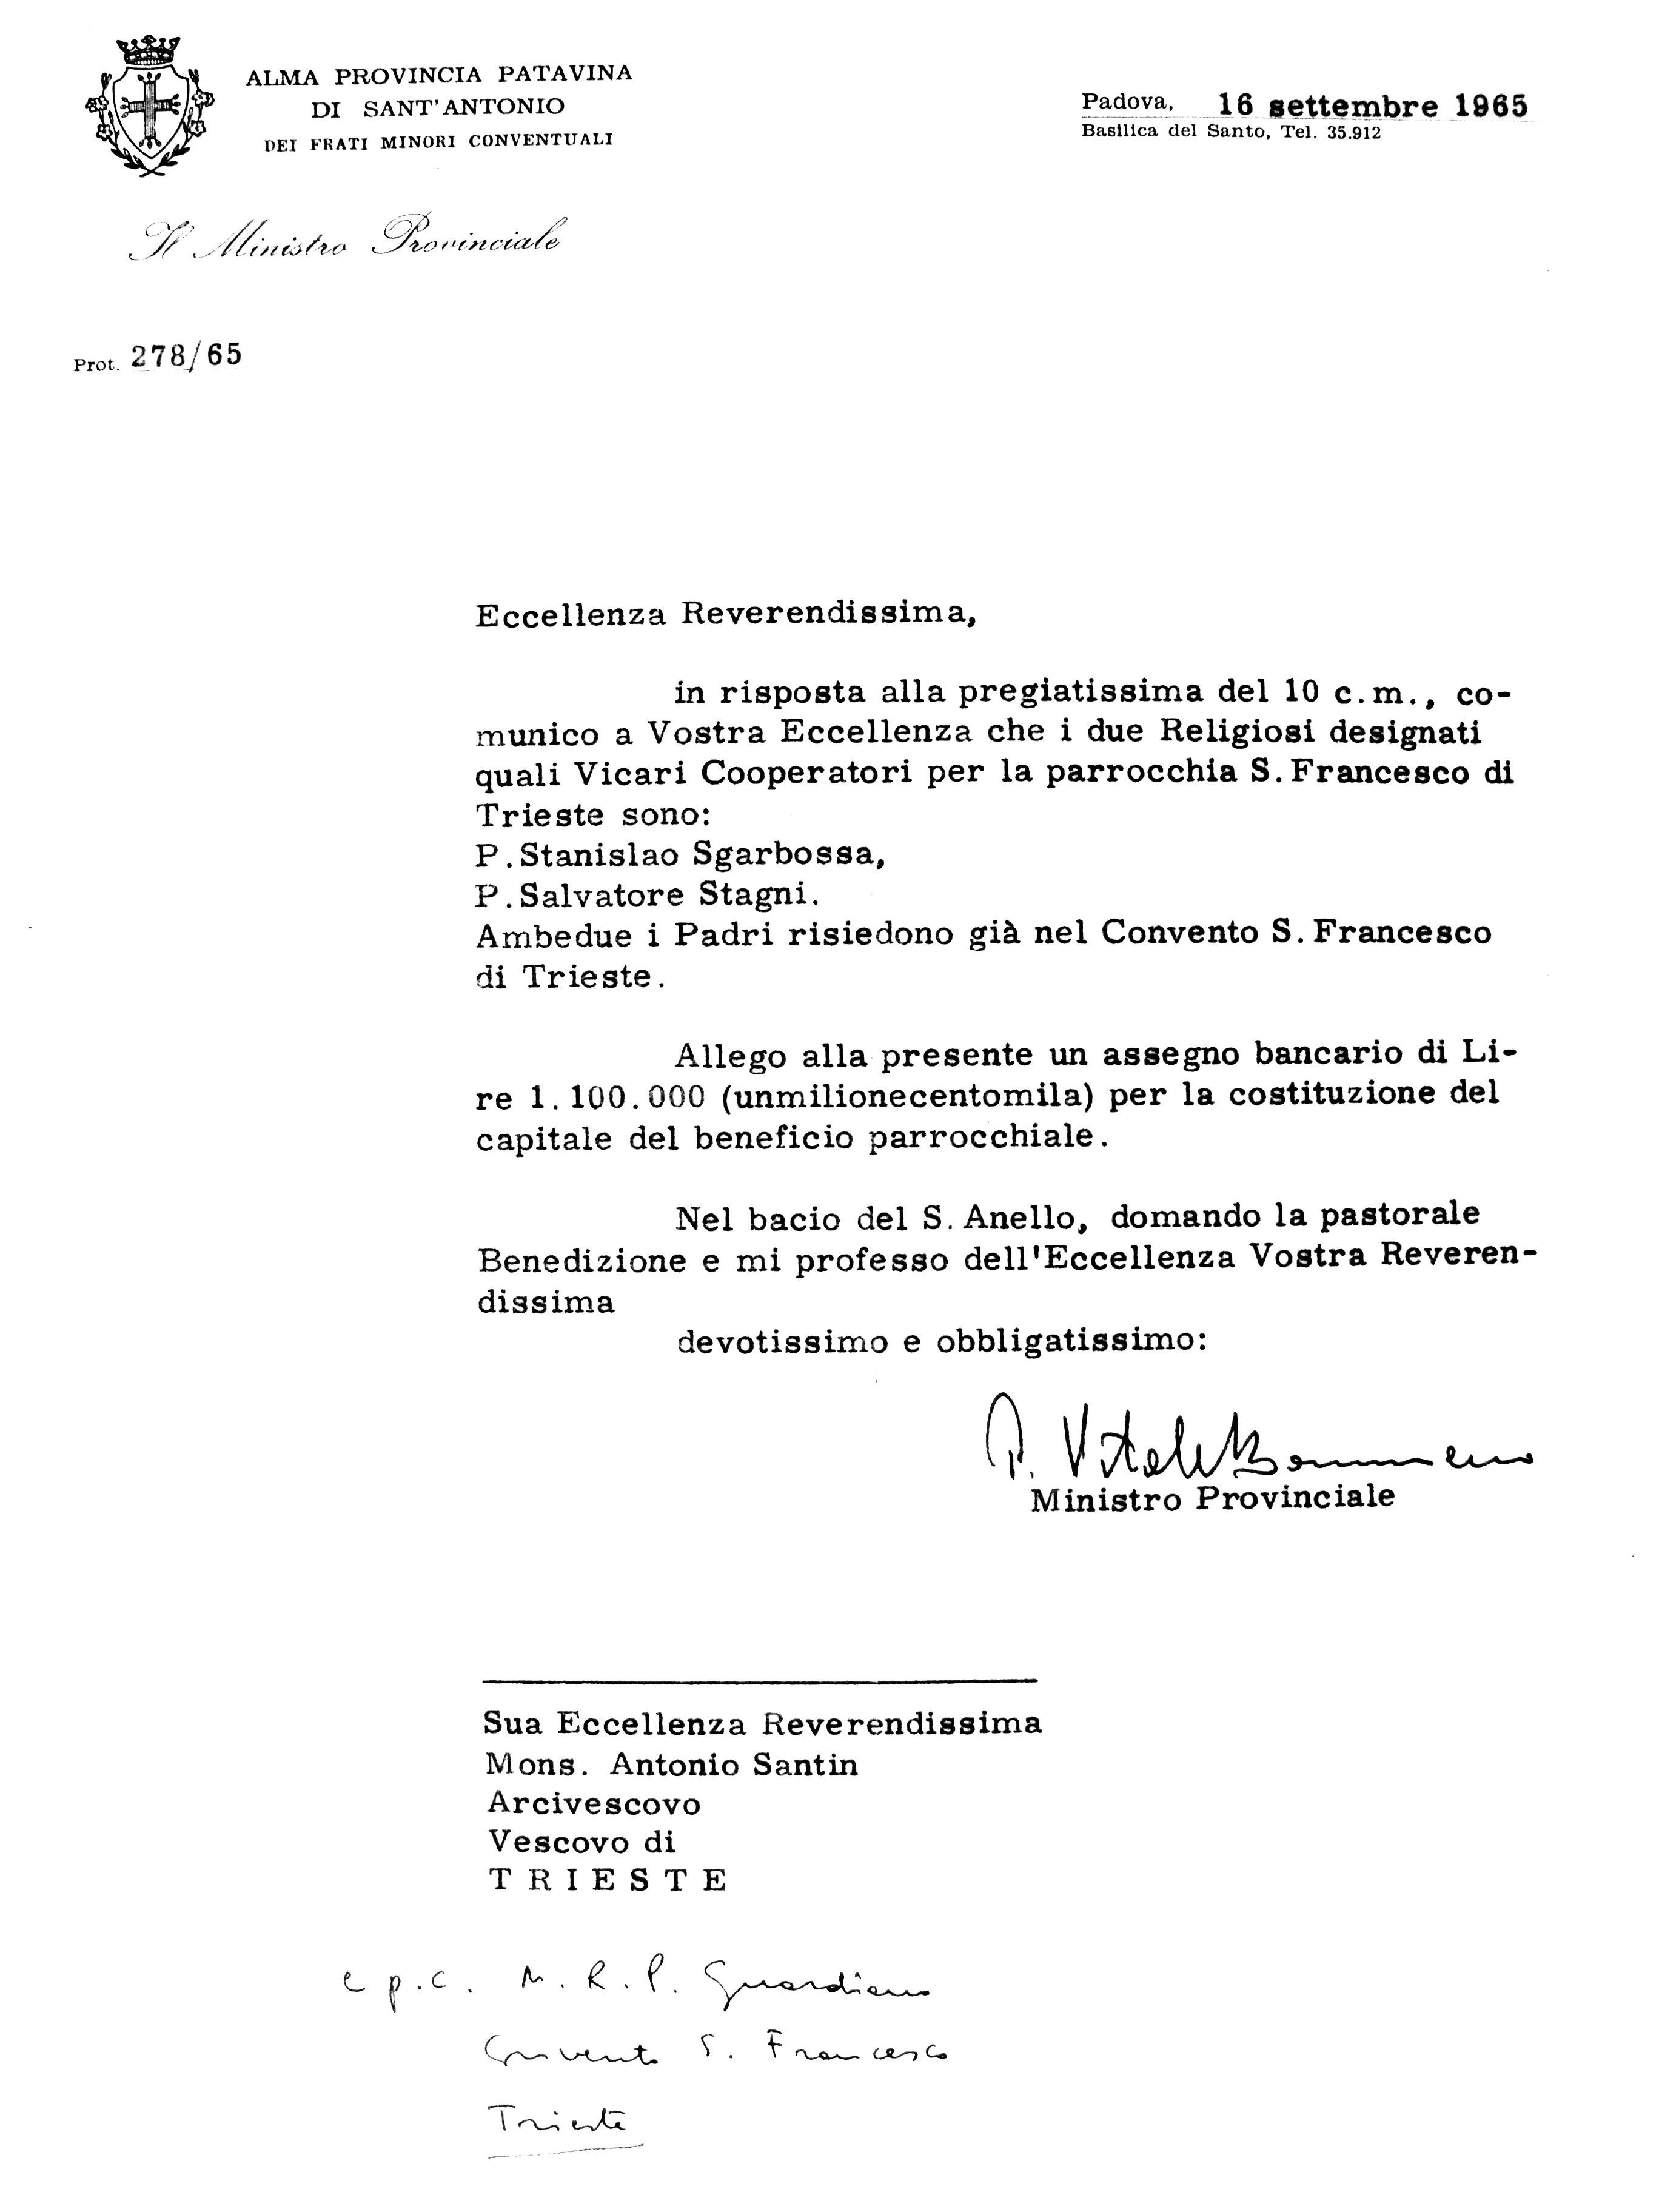
\includegraphics[
	%width=\textwidth,  
	%height=\textheight,
	%]{immagini/i_due_vicari.jpg}%
%\end{center}
%\newpage

\newpage
\begin{center}
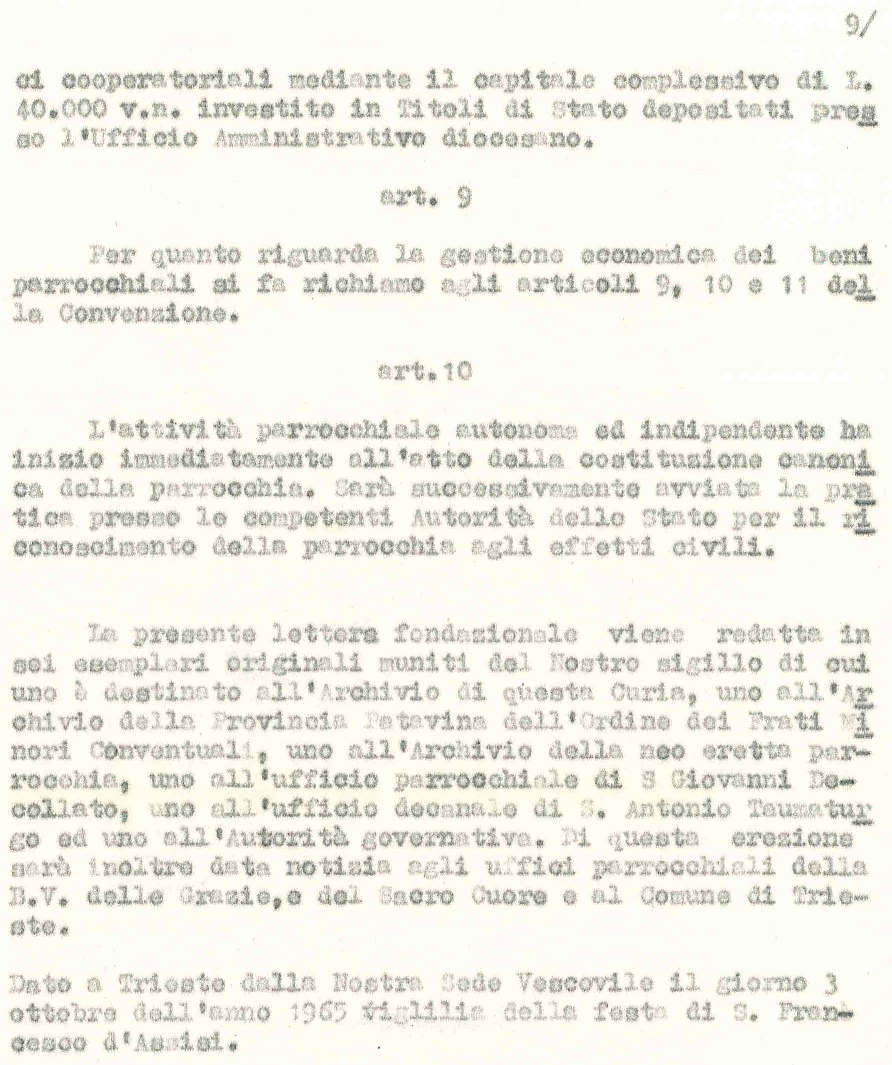
\includegraphics[
	width=1.0\textwidth
	]{testi/lettera_fondazionale10.pdf}%
\end{center}
\vspace*{10mm}
\textit{Il 3 maggio 1994 è stata rinnovata la Convenzione tra la Diocesi di Trieste e la Provincia Patavina OFM Conv (ora Provincia Italiana di S. Antonio di Padova) conforme le nuove indicazioni del Concilio Ecumenico Vaticano II.}

\foreachpage{testi/riconoscimento_civile.pdf}{%
  \newpage   
  \begingroup 
    \centering
    \includegraphics[
      page=\value{imagepage},
      width=\textwidth,  
      height=\textheight,
    ]{testi/riconoscimento_civile.pdf}%
    \newpage
  \endgroup
}

\newpage
\begin{center}
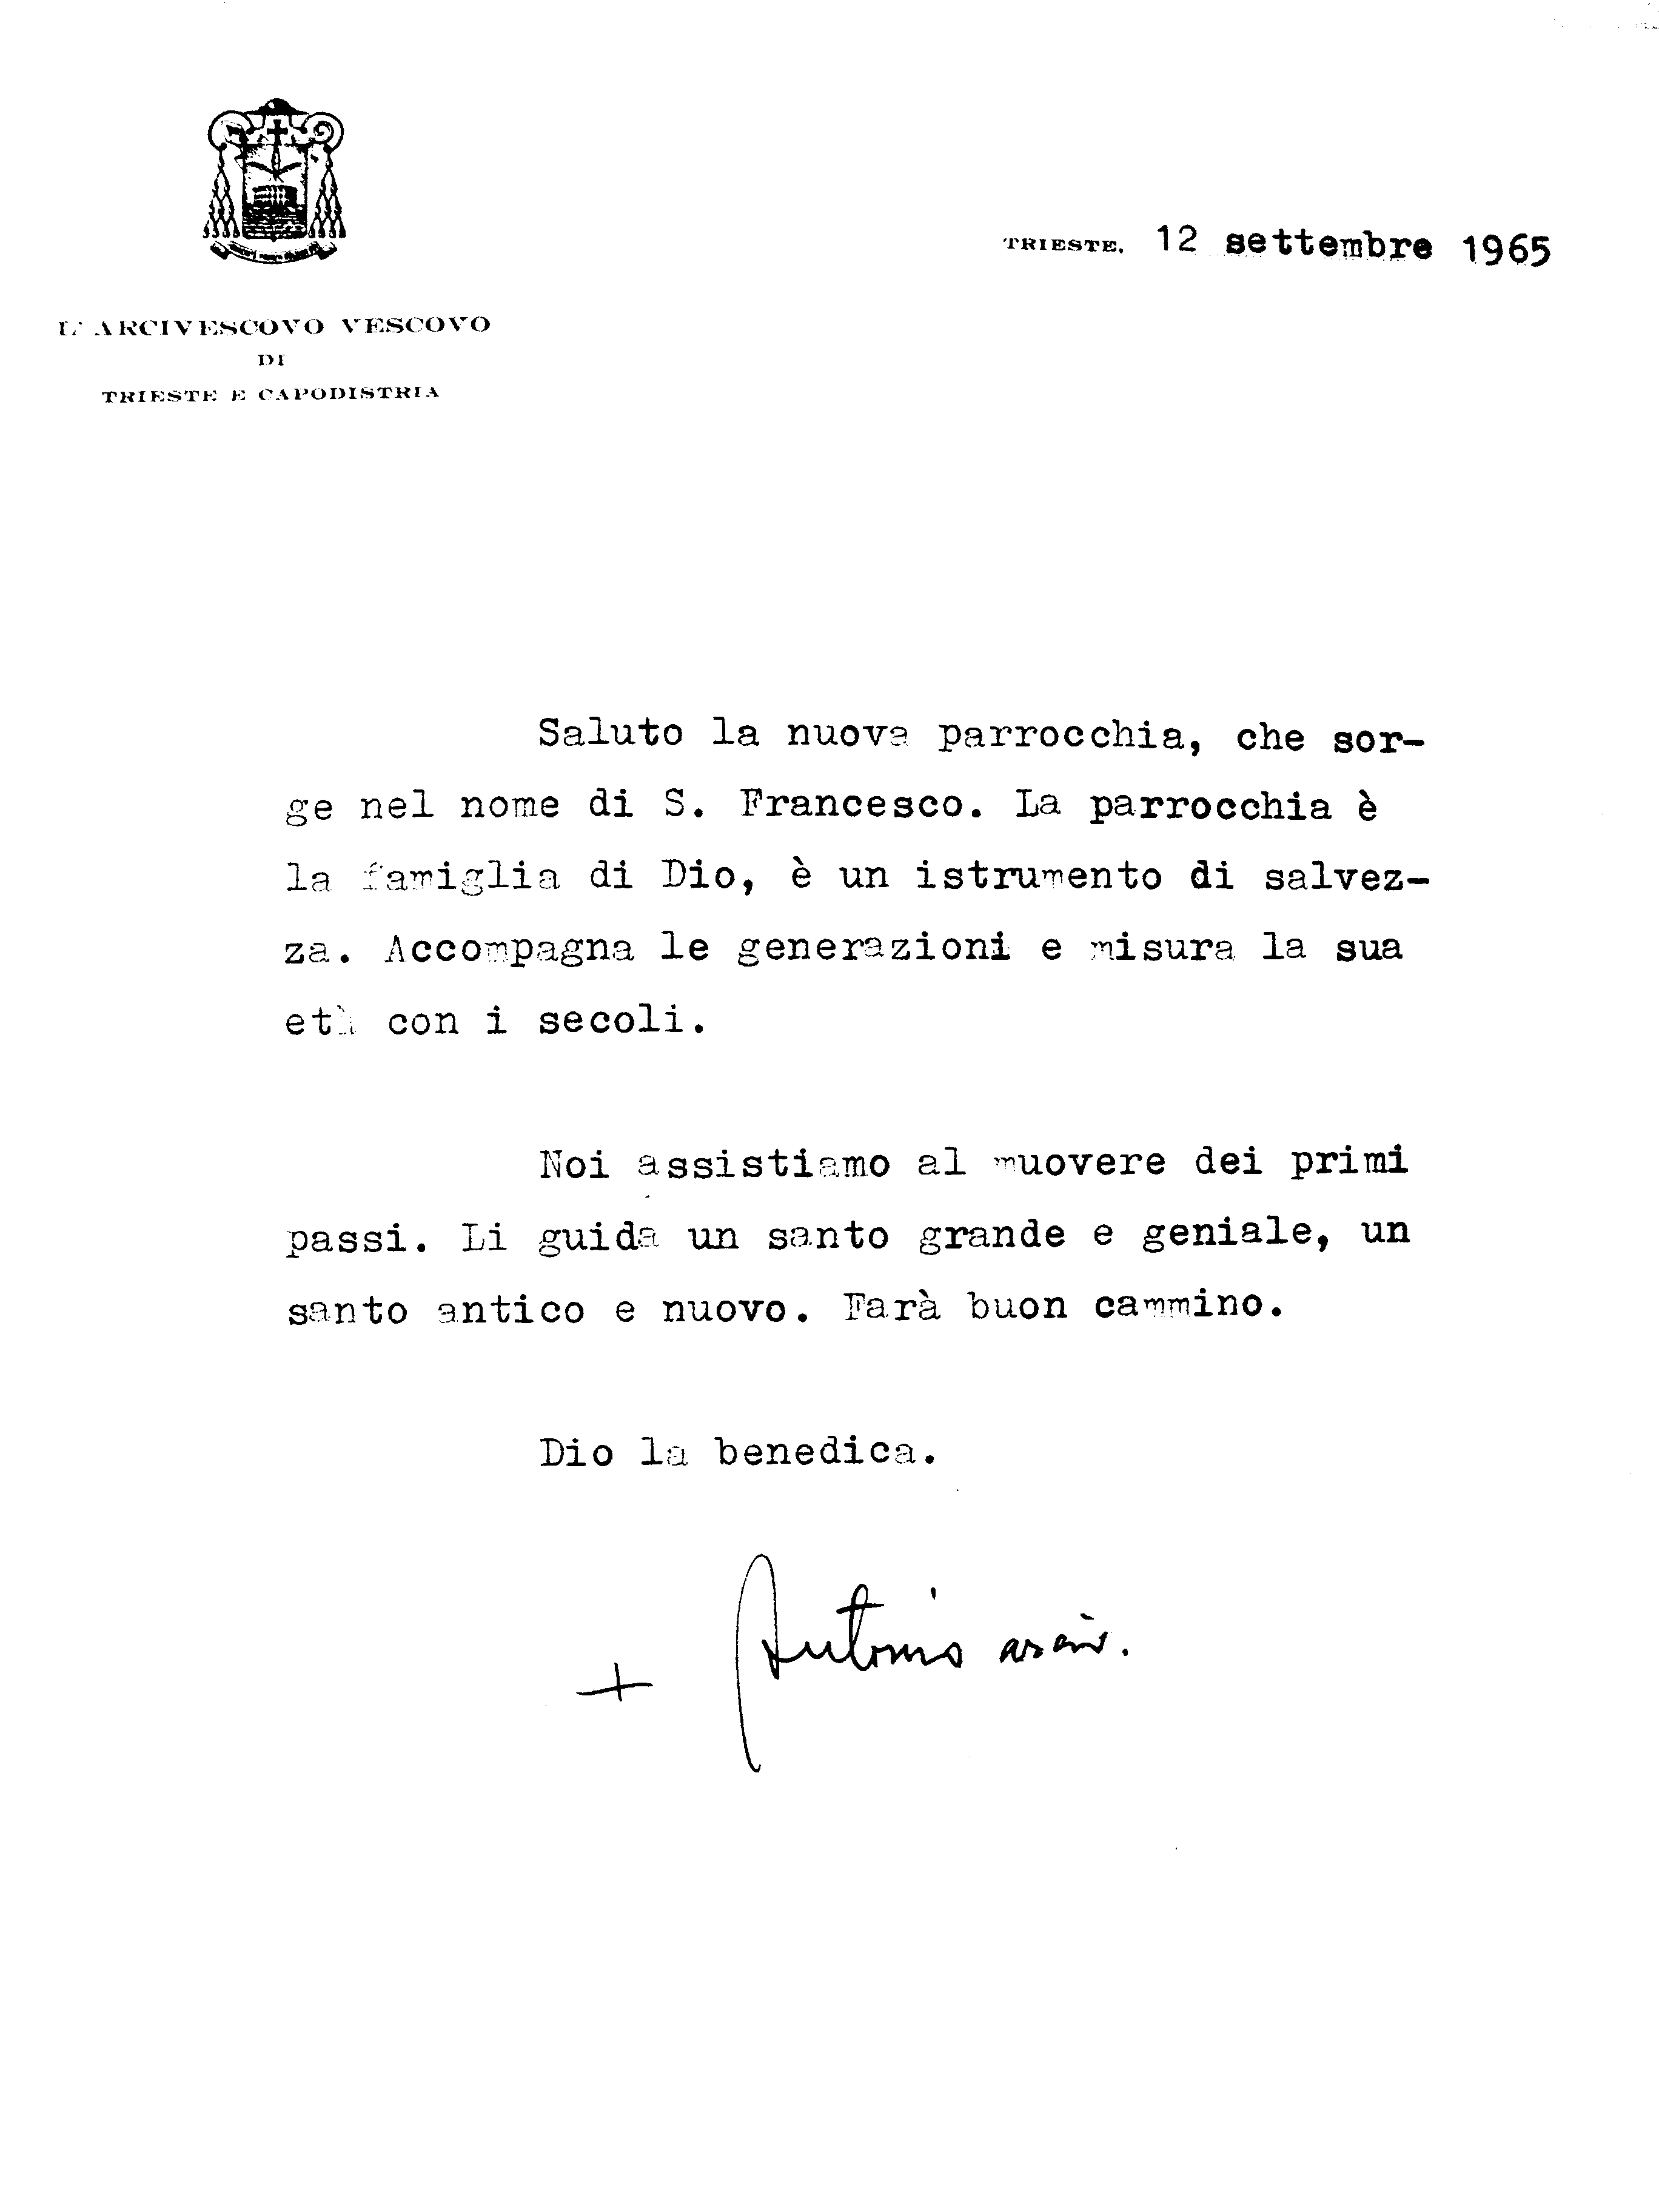
\includegraphics[
	width=\textwidth,  
	height=\textheight
	]{immagini/saluto_dal_vescovo.jpg}%
\end{center}
\newpage
\begin{center}
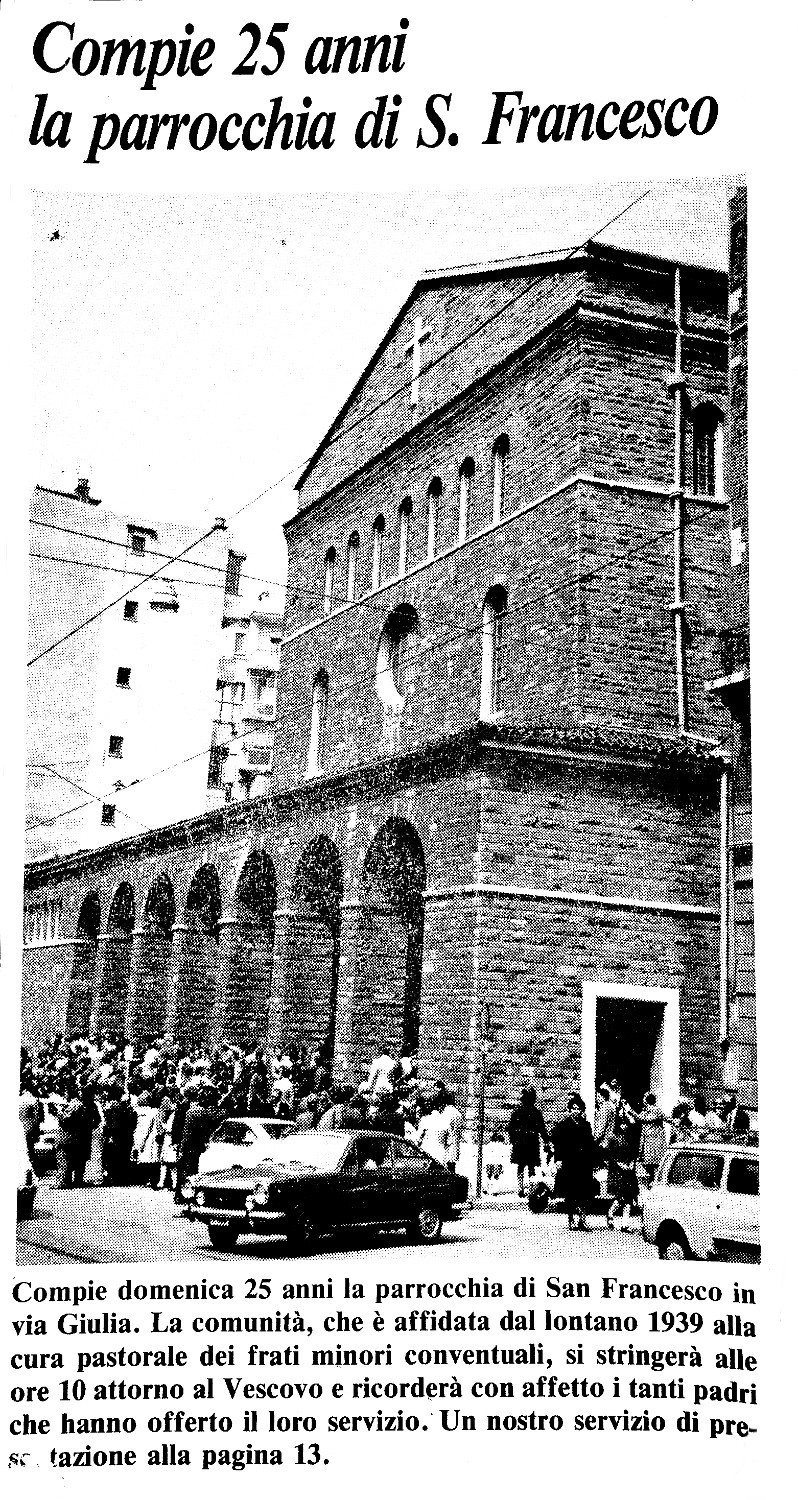
\includegraphics[
	width=\textwidth,  
	height=\textheight,
	keepaspectratio
	]{immagini/FotoParrocchia.jpg}%
\end{center}
\newpage
\chapter{Stradario della Parrocchia}
\label{chap:Stradario}

\begin{center}
\textbf{PARROCCHIA DI SAN FRANCESCO D’ASSISI}\\[0.5cm]
\textbf{STRADARIO 2011}
  %\scriptsize
	\small
	\begin{tabularx}{\textwidth}{| s | s | X |}
		\hline
		\multirow{2}{*}[-0pt]{\textbf{Nome via}} & 
		\textbf{inizio/fine dispari}&\textbf{numeri dispari}\\
		\cline{2-3}
		&\textbf{inizio/fine pari}&\textbf{numeri pari}\\
		\hline
		\multirow{2}{*}[-5pt]{via Berchet} &
		\multirow{2}{*}[-5pt]{tutta} &
		1, 3, 5, 7, 9, 11, 13, 15, 17, 19, 21, 23, 25, 27, 29, 31, 33, 35, 37\\
		\cline{3-3}
		&&2, 4, 6, 8, 10, 12, 12/1, 12/2, 14, 16, 18, 20, 22, 26\\
		\hline
		\multirow{2}{*}{via dei Bonomo} &
		\multirow{2}{*}{tutta} &
		1, 3, 5, 9, 11, 13, 15, 15/1, 17, 19\\
		\cline{3-3}
		&&2, 2/1, 2/2, 2/3, 2/4, 4\\
		\hline
		rotonda del Boschetto&
		tutta meno lato est &
		1, 2, 3, 3/1, 6\\
		\hline
		\multirow{2}{*}{androna Cesarotti} &
		\multirow{2}{*}{tutta} &
		1, 3, 5\\
		\cline{3-3}
		&&2, 4, 6, 8, 10\\
		\hline
		via di Cologna &
		lato dispari fra vie Kandler e Edera &
		25, 27, 27/1, 29, 29/1, 31, 33, 35, 37, 39, 41\\
		\hline
		\multirow{2}{*}{via dei Cunicoli} &
		\multirow{2}{*}{tutta} &
		1, 3, 5, 7, 9, 11, 13\\
		\cline{3-3}
		&&2, 4, 6, 8, 10\\
		\hline
		vicolo dell'Edera &
		dispari inizio via &
		1\\
		\hline
		\multirow{2}{*}{scala Ferolli} &
		\multirow{2}{*}{tutta} &
		1, 3\\
		\cline{3-3}
		&&4\\
		\hline
		\multirow{2}{*}{via Ferrari} & 
		lato dispari tutti&1, 3, 5, 7, 9, 11\\
		\cline{2-3}
		&lato pari inizio via&2\\
		\hline
		\multirow{2}{0.5\linewidth}[-30pt]{\centering via Giulia (finisce in rotonda del Boschetto)} &
		\multirow{2}{0.5\linewidth}[-30pt]{\centering da piazza Volontari Giuliani a fine} &
		41, 43, 45, 47, 49, 51, 53, 55, 57, 59, 61, 63, 65, 67, 69, 71, 73, 75, 75/1, 75/2, 75/3, 77, 79, 81, 83, 85\\
		\cline{3-3}
		&&24, 26, 28, 30, 32, 34, 36, 38, 48, 50, 52, 54, 54/1, 56, 58, 58/1, 60, 62, 64, 66, 68, 70, 72, 74, 76, 78, 80, 82, 84, 86, 88, 90,
		92, 94, 94/1, 96, 96/1, 98, 100, 102, 104, 108\\
		\hline
		\multirow{2}{0.5\linewidth}{\centering via Kandler (finisce in via Giulia) } &
		\multirow{2}{0.5\linewidth}{\centering da via di Cologna a fine} &
		7, 9, 11, 13, 15\bigstrut\\
		\cline{3-3}
		&&8, 10, 12, 14, 16\bigstrut\\
		\hline
		\multirow{2}{*}{via Margherita} &
		\multirow{2}{*}{tutta} &
		1, 5, 7, 9, 11, 13, 15, 19, 21, 23, 25\\
		\cline{3-3}
		&&2, 4, 4/1, 4/2, 4/3, 6, 8, 10\\
		\hline
		\multirow{2}{*}{via Mercantini} &
		\multirow{2}{*}{tutta} &
		1, 3, 5, 7, 9, 11, 11/1, 13\\
		\cline{3-3}
		&&2, 2/1, 4, 6, 8, 10, 12, 14\\
		\hline
		\multirow{2}{*}{scala al Monticello} &
		\multirow{2}{*}{tutta} &
		1, 3\\
		\cline{3-3}
		&&2, 4\\
		\hline
		\multirow{2}{*}{via dell’Oliveto} &
		\multirow{2}{*}{tutta} &
		1, 3, 5, 7, 9, 11\\
		\cline{3-3}
		&&2, 4\\
		\hline
		\multirow{2}{*}{via del Pilone} &
		\multirow{2}{*}{tutta} &
		1, 3, 5\\
		\cline{3-3}
		&&2, 4\\
		\hline
		\multirow{2}{*}[-5pt]{via Pindemonte} &
		\multirow{2}{*}[-5pt]{tutta} &
		1, 3, 5, 5/1, 7, 7/1, 7/2, 7/3, 9, 9/1, 9/2, 9/3, 9/4, 9/5, 11, 13\\
		\cline{3-3}
		&&2, 2/3, 4, 6, 8, 8/1, 8/2, 10, 10/1, 10/2, 12, 14\\
		\hline
		\multirow{2}{*}{via Pisoni} &
		\multirow{2}{*}{tutta} &
		1, 3, 5, 7, 9, 11, 13, 17\\*
		\cline{3-3}
		&&2, 4, 6, 10, 10/1, 12, 14, 18\\
		\hline
		vicolo dei Roveri&
		lato pari &
		2, 4, 6, 8, 10, 14, 16\\
		\hline
		\multirow{2}{*}[-5pt]{androna S. Cilino} &
		\multirow{2}{*}[-5pt]{tutta} &
		1, 3, 5, 7, 9, 11, 13, 15, 17, 19, 21, 23, 25\\
		\cline{3-3}
		&&2, 8, 10, 12, 14, 16, 18, 20, 22, 24, 26, 28, 30\\
		\hline
		\multirow{2}{*}{via S. Cilino} & 
		da inizio a v. S. Primo&1, 3, 5, 7, 9, 11, 13, 21, 23, 25, 27, 29\\
		\cline{2-3}
		&da inizio a v.Roveri&2, 4, 6\\
		\hline
		\multirow{2}{*}{via S. Donato} &
		\multirow{2}{*}{tutta} &
		1, 3, 5, 7, 9, 11, 13, 15, 21, 23\\
		\cline{3-3}
		&&2, 4, 6, 8, 10, 12, 14, 16, 20, 24, 26, 28\\
		\hline
		\multirow{2}{*}{via S. Felice} &
		\multirow{2}{*}{tutta} &
		1, 3, 5, 7\\
		\cline{3-3}
		&&2, 4, 6, 8, 10, 12, 14, 16\\
		\hline
		campo S. Luigi&
		lato v. Pindemonte &
		1, 1/1, 2, 3, 3/1, 4, 5, 6, 7\\
		\hline
		scala S. Luigi&
		lato pari&
		2\\
		\hline
		via S. Primo&
		dispari inizio via&
		1\\
		\hline
		\multirow{2}{0.5\linewidth}[-5pt]{\centering pendice dello Scoglietto} & 
		lato dispari tutti&1, 3, 3/1, 3/2, 5, 5/1, 5/2, 5/3, 5/4, 5/5, 5/6, 7, 7/1, 9, 11, 13, 13/1, 15, 17\\*
		\cline{2-3}
		&lato pari da inizio a vicolo dell’Edera&2, 4, 6, 8, 10, 12, 14, 16, 18\\
		\hline
		\multirow{2}{0.5\linewidth}{\centering via dello Scoglio (inizia in via Giulia)} &
		\multirow{2}{0.5\linewidth}{\centering da inizio a pendice Scoglietto} &
		1, 3, 5, 7, 9, 11, 13, 15, 17, 19, 21, 23, 25, 27, 29, 31, 33, 35, 37, 39, 51, 59, 61, 63, 67, 69, 71, 73, 75, 77, 83, 85, 87, 89, 
		91, 95, 97, 99, 103, 1077\\*
		\cline{3-3}
		&&2, 4, 6, 8, 12, 14, 14/1, 16, 18, 20\\
		\hline
		\multirow{2}{0.5\linewidth}[-5pt]{\centering viale XX Settembre (finisce in via Bonomo)} &
		\multirow{2}{0.5\linewidth}[-5pt]{\centering da piazza Volontari Giuliani a fine} &
		77, 79, 81, 83, 85, 87, 89, 89/1, 93, 97, 97/1, 101, 103\\*
		\cline{3-3}
		&&72, 74, 76, 78, 80, 82, 84, 86, 88, 90, 92, 94, 96, 98, 100, 100/1, 102, 102/1, 104\\
		\hline
		\multirow{2}{*}[-15pt]{via Verga} & 
		lato dispari tutti&1, 3, 9, 11, 13, 15, 17, 19\\
		\cline{2-3}
		&lato pari da inizio a via Zanella&2, 4, 6, 8, 8/1, 10, 12, 14, 16, 16/1, 18, 20, 20/2, 20/3, 22, 24, 26, 28, 30, 32, 34, 36, 38, 40,
		42, 42/1, 44, 44/1, 46, 48, 50, 52, 54, 56, 58\\
		\hline
		piazza Volontari Giuliani&
		tutta tolto lato ovest&
		1, 2, 3, 4, 5, 6, 7, 8\\
		\hline
		via Zanella&
		lato dispari da androna Cesarotti a fine (eccetto 129)&
		29, 31, 33, 35, 37, 41, 43, 45, 47, 49, 51, 53, 55, 57, 59, 61, 63, 65, 67, 69, 71, 73, 75, 77, 79, 81, 83, 85, 87, 89, 91, 95, 97, 99, 
		101, 103, 105, 107, 109, 111, 113, 115, 117, 119, 121, 123, 127\\
		\hline
	\end{tabularx}
\end{center}
\begin{center}
\needspace{3\baselineskip}
\textbf{NUMERI ANAGRAFICI}
  %\scriptsize
	\small
	\begin{tabularx}{\textwidth}{| s | X |}
		\hline
		località Chiadino&
		867\\
		\hline
		località Città&
		4922 (chiesa)\\
		\hline
	\end{tabularx}
\end{center}
\begin{center}
\textbf{VIE SENZA NUMERI}
  %\scriptsize
	\small
	\begin{tabularx}{\textwidth}{| s | X |}
		\hline
		piazzale Dreher&
		tra le vie Bonomo, Pindemonte, Giulia\\
		\hline
		bosco dei Pini&\\
		\hline
	\end{tabularx}
\end{center}
\begin{figure}[h]
\centering
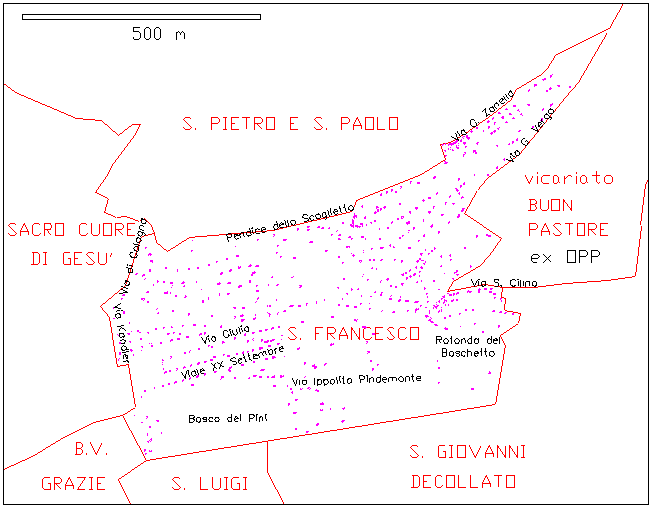
\includegraphics[
	width=0.8\textwidth
	]{immagini/mappa.png}%
\caption{Mappa della parrocchia di San Francesco.}
\end{figure}
\chapter{I Parroci raccontano}
\label{chap:Testimonianze}

\begin{center}
\textbf{\Large p. FORTUNATO ZORZINI}\\
	\textit{Amministratore parrocchiale dal 1965 al 1967}
\end{center}
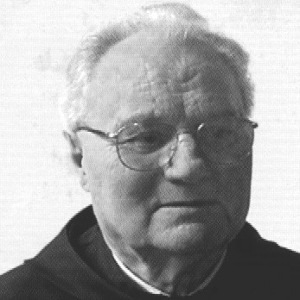
\includegraphics[width=0.31\textwidth]{immagini/zorzini.jpg}
\bigskip
\begin{center}
\textbf{\Large p. OLINDO BALDASSA}\\
	\textit{parroco dal 1967 al 1976}
\end{center}
%\textbf{Vicari: p. Stanislao Sgarbossa e p. Salvatore Stagni}
\bigbreak
\begingroup
\setlength\intextsep{0pt}
\begin{wrapfigure}[7]{l}{0.31\textwidth}
\centering
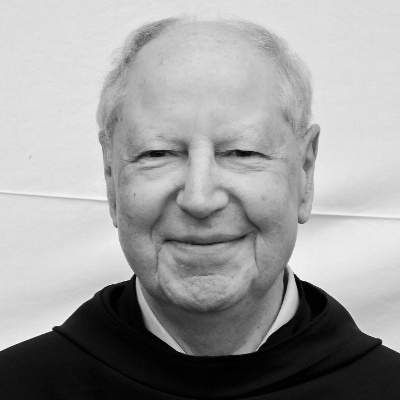
\includegraphics[width=0.31\textwidth]{immagini/olindo.jpg}
\end{wrapfigure}
\noindent Nel mio pro-memoria per il Cinquantesimo di ordinazione sacerdotale (2010) “Cinquant’anni di grazia. (spigolature)” riferendomi ai nove anni di attività pastorale nella parrocchia di s. Francesco di Trieste (1967 – 1976) mi ero espresso in questo modo:
\bigbreak 
\enquote{\itshape Quel po' di esperienza pastorale fatta presso la parrocchia dei santi Pietro e Paolo all’Eur (Roma) ancora fresco di ordinazione, e quella acquisita nella direzione dei chierici, sono venute buone quando i superiori mi hanno assegnato al convento di s. Francesco d’Assisi di Trieste con il duplice compito di superiore dei frati e di parroco della parrocchia dal vescovo assegnata ai religiosi conventuali.

Quella triestina è stata una stagione pastoralmente splendida, indimenticabile. Le primizie, infatti, sono sempre deliziose e piacevoli. Dal punto di vista canonico sono stato il primo religioso della comunità a ricoprire il ruolo di parroco della parrocchia triestina di s. Francesco. Se l’esperienza è stata positiva, e non solo per me, lo devo anche alla benevolenza del vescovo, monsignor Antonio Santin, alla cordialità dei sacerdoti diocesani e dei religiosi miei confratelli e, soprattutto, all’amicizia e all’affetto dei parrocchiani, che rimangono come perle preziose incastonate nella collana dei miei giorni. 

Trieste, città di confine e mitteleuropea, è sempre stata sensibile all’approccio ecumenico con altre esperienze religiose vicine e lontane: un percorso nel quale anche la nostra comunità si è efficacemente inserita, con varie iniziative.

Su altro versante, è stato impegnativo ma gratificante, il lavoro di rifacimento dell’interno della chiesa, con la rimozione dell’intonaco da tutta la superficie per liberare la pietra faccia a vista, che ha dato all’edificio un volto nuovo e con il rinnovato impianto di illuminazione, quasi anticipo e preludio dei successivi lavori, pure molto impegnativi, di sistemazione di tutta l’area presbiteriale. 

Del periodo triestino mi piace segnalare alcuni avvenimenti particolari, ancora vivi nel ricordo, come il viaggio ecumenico della diocesi a Istanbul, guidato da monsignor Santin e don Eugenio Ravignani, culminato nell’incontro con il Patriarca ortodosso Athenagoras I e il mio primo pellegrinaggio in Terra Santa, nel 1973, offertomi dai parrocchiani.}
\bigbreak

Vengo ora a ripetere e rinnovare gli stessi sentimenti anche in questa circostanza, aggiungendovi qualche nota. 

Il decreto canonico di erezione a parrocchia veniva a confermare quanto già da circa venti anni si svolgeva in quella zona dello Scoglietto – Guardiella con il ritorno dei Frati Minori Conventuali. 

Non è stato perciò difficile inserirmi in quel contesto così bene avviato e consolidato con tutte le attività proprie di una comunità cristiana già ben collocata nel territorio diocesano. Preziosa la collaborazione con le Suore Dimesse. Cura e premura particolari del parroco si sono subito rivolte alla conoscenza diretta e personale nella fatica e nella gioia della benedizione e incontri familiari… 

Siamo agli inizi della riforma liturgica e della ripresa del cammino ecumenico: fare della parrocchia una comunità alimentata dalla liturgia feriale e festiva, curando specialmente le celebrazioni comunitarie dei battesimi, anniversari di matrimonio, prime comunioni, cresime, prime messe dei sacerdoti novelli dell’Istituto Teologico di Padova, fioretto di Maggio all’altare della Madonna con uno stuolo di irrequieti chierichetti o nei vari cortili in mezzo alle abitazioni, il pellegrinaggio annuale al santuario di Monte Grisa… e altri incontri di spiritualità e condivisione…. Un capitolo particolare merita la cura e attenzione all’oratorio per i ragazzi e i giovani. 

I sentimenti che hanno riempito la mia stagione pastorale triestina sono stati di dialogo, rispetto, collaborazione, fraternità e sincera amicizia, largamente ricambiati. Di tutto questo ancora ringrazio il Signore e auguro alla Comunità religiosa e parrocchiale di proseguire con lena sulla strada della nuova evangelizzazione secondo le incalzanti indicazioni di Papa Francesco. 
\begin{flushright}
\textit{P. Olindo M. Baldassa}
\end{flushright}
\endgroup
\begin{center}
	\noindent\rule{\textwidth}{0.4pt}
\end{center}
\textit{Riteniamo utile, a completamento di quanto ci ha raccontato p. Olindo, riportare il suo saluto alla parrocchia, nel giorno della sua partenza:}
\bigskip
\begin{flushright}
Trieste, 3 ottobre 1976
\end{flushright}
Miei Fratelli,
\smallbreak
la domenica 15 Ottobre 1967 mi presentavo a voi assumendo il servizio pastorale di questa comunità parrocchiale, oggi celebro per voi e con voi la S. Messa passando ad altre mani il mio mandato.
Sono passati 9 anni: possono essere considerati molti o pochi a seconda del punto di vista dal quale ci si colloca, è un normale avvicendamento, sia pure non richiesto, sono stati comunque vissuti 
questi nove anni, mi sembra di poter dire con intensità di operosità, di conoscenza reciproca, di stima, di crescita nella comune vocazione alla risposta della parola di Dio.
Mi sia consentito, sia pure brevemente, di ricordare qualche tratto del cammino svolto insieme in questi anni:
in continuità di opere con il mio predecessore mi sono anzitutto dedicato a rendere sempre più accogliente la chiesa, come luogo di riunione e convegno di preghiera: 
ecco i banchi nuovi offerti in memoria dei vostri defunti, le suppellettili e arredi per una nobile e dignitosa celebrazione delle sacre funzioni, il riscaldamento della chiesa esteso anche al 
Franciscanum e Oratorio, il rimaneggiamento della pavimentazione, la ristrutturazione dell’impianto di illuminazione e i sei grandi pendenti, l’impianto di amplificazione e finalmente
il grande, lungo, faticoso restauro della superficie muraria interna con la demolizione degli intonaci e la pulitura delle superfici dei conci di pietra arenaria e successiva fugatura così
da portare a vista tutta la superficie interna e dare un volto nuovo, vibrante e austero, a tutta l'architettura e significare così, almeno per immagine, la vera struttura della chiesa, corpo
mistico di Cristo, costituita da pietre vive.
La non indifferente somma di denaro per far fronte e sostenere le spese per detti lavori è stata, reperibile grazie alla alla vostra generosità e ad una accorta amministrazione senza lasciare
attualmente alcuna passività.
Ma la mia cura maggiore si è rivolta non tanto alle opere da fare, sia pure utili o necessarie, quanto alle persone come componenti vive della comunità cristiana dirigendo in particolare 
la mia azione verso il ministero di\\
a) dispensatore della parola intesa come evangelizzazione, infatti quante prediche avete sentito... e le istruzioni nelle diverse Associazioni (Azione Cattolica, Terz'Ordine, Milizia, 
S. Vincenzo, giornate particolari con tridui, novene ecc.... assemblee, incontri di mamme e papà ... e la preparazione catechistica ai bambini per i sacramenti della iniziazione cristiana e 
agli adulti per vivificare il senso di consapevolezza e responsabilità dei loro doveri cristiani nei confronti dei figli....da questa maturazione ecco l'aspetto di\\
b) dispensatore dei sacramenti: come veri incontri con la grazia di Dio che fa rinascere nel battesimo, corrobora nella Cresima, nutre nell'Eucarestia, perdona nella riconciliazione, 
consacra l'amore nel matrimonio, risana e apre a speranza nell'unzione degli infermi.\\Lo sforzo ancora e l'impegno all'interno di questa famiglia di farmi\\
c) dispensatore di carità, nell'accoglienza e nel servizio tutte le persone nelle visite alle famiglie; gli ammalati e i vecchi in modo particolare, nella preghiera fatta insieme qui in chiesa,
nelle vostre abitazioni e anche nei vostri cortili come non ricordare il maggio dell'anno scorso, l'anno santo, e l'attenzione ecumenica fatta di conoscenza 
e rispettosa deferenza verso i Fratelli separati...\\
Intenzione esplicita e come forza motrice in questi anni mi è stata quella di creare tra noi tutti un clima di famiglia, rendere la chiesa veramente la casa di tutti, la casa comune, dove ognuno si
sentisse a suo agio, si sentisse bene, e vi potesse aprire serenamente e fiduciosamente il suo animo e ...
quindi le Associazioni Cattoliche sì, ma volutamente non ho prestato attenzione a gruppi o gruppuscoli che avessero potuto essere elementi di separazione e di isolamento nel tessuto della
comunità. Con particolare predilezione ho curato i chierichetti, sempre bravi e numerosi alle celebrazioni; il settore giovani è stato quello che per diverse cause, 
sia logistiche di spazi e ambienti che per mancanze di personale ha più sofferto.
Ai momento quindi di accomiatarmi, ringrazio tutti voi per le preziose e attente collaborazione prestate, a sviluppare questi miei intendimenti che il Signore Dio giudicherà nella 
loro realizzazione.
Essendo la parrocchia una parte della chiesa locale ossia della Diocesi rivolgo il mio deferente pensiero al Vescovo che ora la governa e in particolare a Mons. Santin con il quale
ho maggiormente intrattenuto relazioni di collaborazione e di rispettosa e filiale vicinanza.
È per me doveroso ricordare e accomunare nel ringraziamento tutti i confratelli che hanno con me condiviso in questi anni (anche se ora si trovano lontano da noi) 
la responsabilità e le fatiche dell'apostolato nei diversi settori pastorali e qui rappresentati nella concelebrazione da P. Luigi... 
Il mio successore: non spetta a me presentarlo, lo farà ufficialmente il Vescovo domani durante la Messa Vespertina; mi sia consentito solamente di dire che egli viene in mezzo a voi ricco di
esperienza pastorale avendo già retto per undici anni la parrocchia del Tempio Votivo a Verona, e secondariamente, un fatto personale: il P. Innocenzo era allora sacerdote novello a 
Camposampiero e per quei miei primi anni di Seminario è stato il mio Direttore Spirituale...una certa continuità...
\begin{flushright}

\includegraphics[scale=0.16]{immagini/firmaBaldassa.jpg}
\end{flushright}
%\newpage
\newpage
\begin{center}
\textbf{\Large p. INNOCENZO BORDIN}\\
	\textit{parroco dal 1976 al 1985}
\end{center}
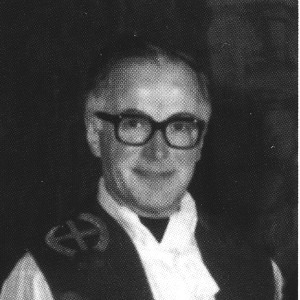
\includegraphics[width=0.31\textwidth]{immagini/bordin.jpg}
\vfill
\begin{center}
\textbf{\Large p. GERMANO BUSO}\\
	\textit{parroco dal 1985 al 1988}
\end{center}
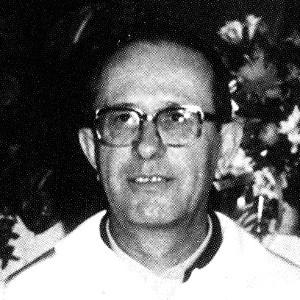
\includegraphics[width=0.31\textwidth]{immagini/buso.jpg}
\vfill
\newpage
\begin{center}
\textbf{\Large p. LORENZO GOTTARDELLO}\\
	\textit{parroco dal 1988 al 1997}
\end{center}
\bigbreak
\begingroup
\setlength\intextsep{0pt}
\begin{wrapfigure}[7]{l}{0.30\textwidth}
\centering
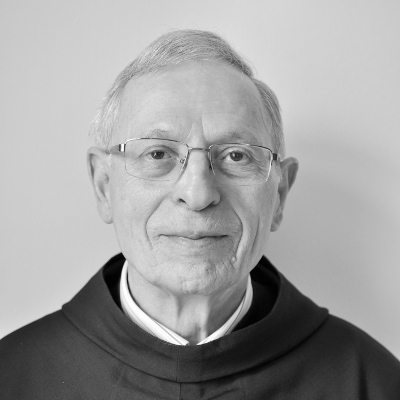
\includegraphics[width=0.30\textwidth]{immagini/lorenzo.jpg}
\end{wrapfigure}
\noindent \textit{Qualche traccia del mio vissuto a Trieste}
\medbreak
\noindent Provo mettere per iscritto qualcosa di quanto rimane in me, dopo molti anni, della mia
esperienza vissuta nella comunità parrocchiale di San Francesco in via Giulia. 
Non intendo stendere una cronaca, ma far emergere dalla mia memoria tracce che ritrovo ancora 
tanto vive di quel tempo trascorso a Trieste nella sezione di tempo: 1988-1997.
Avevo 52 anni quando approdai a Trieste. Venivo dall’esperienza pastorale romana protrattasi dal 
1973 al 1988 nella parrocchia di S. Marco, prima, e poi nella nuova parrocchia di S. Giuseppe da 
Copertino.
Non conoscevo per niente Trieste, né la realtà pastorale di S. Francesco. Conoscevo però i 
frati presenti allora: p. Tarcisio (per tutti: Ciccio); p. Luigi con cui avevo condiviso un anno a 
Roma; p. Giovanni, mio compagno di seminario; non conoscevo, se non di nome, il più giovane 
della comunità: p. Giambattista Bontempi.
Mi sentivo mandato dai superiori ad essere “guardiano” dei frati per essere insieme un segno di 
presenza francescana secondo l'ideale di San Francesco. In secondo luogo mi sentivo parroco 
inviato dal Vescovo per essere animatore e coordinatore delle attività pastorali nella parrocchia di 
San Francesco insieme con gli altri miei confratelli.
Nell'arco del mio mandato c'è stato un inserimento nuovo e alcuni avvicendamenti nella 
comunità dei frati. Nell'ottobre '89 è arrivato fra Armando con il compito di sacrestano e di prima 
accoglienza delle persone in sacrestia. Nel settembre '91 p. Giovanni, dopo 12 anni di permanenza è 
destinato a Sabaudia. Arriva in sostituzione numerica p. Adolfo della Torre: una meteora che 
compare solo per un anno. Così nel '92 arriva p. Ruggero Lotto desideroso di reinserirsi nella 
pastorale parrocchiale, mentre  è del novembre '93 la irremovibile scelta di p. Bontempi di andare a 
svolgere il suo ministero pastorale alla dipendenza di un vescovo diocesano. La sua partenza ha 
creato un vuoto pastorale in oratorio e tante difficoltà nel portare avanti l'animazione in quel settore. 
Nel settembre '94 il p. Provinciale ci ha inviato il giovane diacono p. Enzo Piovesan per prendere in 
mano la realtà dell'oratorio e l'animazione della pastorale giovanile. 
E' chiaro che ogni partenza lascia un po' di vuoto e ogni arrivo va accolto con le caratteristiche e 
propensioni pastorali che ognuno porta con sé, e questo richiede attenzione da parte di tutti per 
creare un nuovo spirito e un nuovo gioco di squadra.
\bigbreak
\needspace{3\baselineskip}
\noindent\underline{La Missione al popolo}
\medbreak
\noindent Quando sono arrivato a Trieste la diocesi era tutta presa dall'impegno della preparazione, 
ormai prossima, della Missione al popolo, che si è svolta poi in tutte le parrocchie dal 12 al 26 
febbraio '89.
Circa 400 missionari hanno ricevuto dal vescovo il crocefisso e sono stati inviati nelle varie 
parrocchie e realtà pastorali della diocesi per ravvivare la fede del popolo cristiano. Nella nostra 
parrocchia sono stati accolti e ospitati sette missionari: tre nostri confratelli e quattro suore 
francescane. Il coordinatore era il p. Francesco Faldani, già espulso dalla Cina e fondatore della 
missione in Corea. Nella prima settimana hanno visitato le famiglie riportando giorno per giorno 
informazione, richieste di vario genere e disponibilità a partecipare a cammini formativi e a servizi 
di volontariato nella comunità. Nella seconda settimana i missionari si sono concentrati nelle 
celebrazioni in chiesa e nelle catechesi comunitarie per raggruppamenti diversi, secondo le età.
Sono stati 15 giorni di presenza particolare dello Spirito Santo che ha ravvivato la fede nel 
cuore di molti. Frutto della Missione al popolo è stata la nascita di diversi gruppi di ascolto della 
Parola presso le famiglie e poi l'incontro settimanale sui testi biblici per celebrare l'eucarestia 
domenicale in maniera più partecipata e fruttuosa.
\bigbreak
\needspace{3\baselineskip}
\noindent \underline{Cammino neocatecumenale}
\medbreak
\noindent Prosperava in parrocchia da diversi anni la presenza del cammino neocatecumenale capace 
di avvicinare i lontani e di proporre un percorso impegnato attorno alla Parola, nella celebrazione 
viva dei sacramenti e nella carità, per essere poi annunciatori di Cristo a tutti gli uomini. Era una 
esperienza particolare che non poteva però proporsi come l'unica realtà della comunità parrocchiale, 
né d'altra parte porsi come cammino parallelo accanto a quello ordinario della comunità. 
Proprio alla fine della Missione al popolo e all'inizio del cammino verso la Pasqua il pastore 
della diocesi, il vescovo mons. Lorenzo Bellomi, ha emanato “Le Norme per il cammino 
neocatecumenale” da osservarsi in diocesi. Queste sono diventate da subito mio riferimento 
pastorale nei confronti del cammino in parrocchia. Le norme non sono mai state ufficialmente 
revocate. Le forti pressioni delle alte gerarchie dei neocatecumenali hanno indotto il Vescovo 
tacitamente a congelare tali Norme...
Con i responsabili del cammino neocatecumenale a San Francesco ci sono state diverse tensioni. 
Quando è intervenuto il loro grado gerarchico di livello superiore ho chiesto che mettessero in 
iscritto i punti essenziali per continuare il cammino in San Francesco, ai quali avrei data risposta 
scritta. Sul tenore della mia risposta i responsabili del Cammino neocatecumenale hanno deciso di 
spostare le comunità altrove. Il Vescovo Lorenzo Bellomi non mi ha mai mosso alcun rimprovero 
sul mio atteggiamento fermo, tenuto nei confronti del cammino neocatecumenale; d'altra parte gli 
avevo detto, dopo la confusione creatasi, che avrei agito decisamente secondo la mia coscienza.
\bigbreak
\needspace{3\baselineskip}
\noindent \underline{Coloritura francescana della parrocchia}
\medbreak
\noindent Dopo la Missione al popolo, oltre che impegnarci nel mettere al centro la Parola di Dio nel 
cammino della comunità, abbiamo incominciato a riflettere sulla coloritura francescana che doveva 
avere la parrocchia di San Francesco: perché era sotto la protezione del santo patrono d'Italia,  
perché era affidata ad una comunità di frati francescani, perché al suo interno aveva già altre piccole 
presenze francescane come la GIFRA e l'OFS che potevano essere sviluppate. Così abbiamo 
improntato un cammino di sensibilizzazione francescana durato diversi mesi. Nel contesto di questo 
percorso francescano abbiamo partecipato come parrocchia al grande pellegrinaggio regionale in 
Assisi, il 4 ottobre, per l'offerta dell'olio per la lampada votiva; abbiamo iniziato un cammino di 
formazione specifica per entrare nell'OFS e infine il 28 ottobre '90 abbiamo ricordato il 25\textdegree\ della 
parrocchia, che ricorreva il 3 ottobre, quando eravamo in pellegrinaggio in Assisi. 
C'è stato un triduo di preparazione; in una serata il p. Provinciale, p. Agostino Gardin 
(attuale vescovo di Treviso), ha sviluppato il tema: “Caratteristiche di una parrocchia animata da 
frati francescani”. 
Domenica 28 ottobre con semplicità abbiamo ricordato i 25 anni di vita della parrocchia con la 
presenza del vescovo mons. Lorenzo Bellomi, dei due ex parroci viventi: p. Fortunato e p. Olindo e 
dei sacerdoti del decanato. Al termine della Messa solenne il Vescovo ha benedetta la rinnovata 
sede della Fraternitas e i nuovi impianti sportivi, completamente rinnovati grazie alla tenacia di p. 
Giambattista. 
Circa la coloritura francescana della comunità parrocchiale successivamente è stata ripresa la 
Milizia dell’Immacolata (di p. Kolbe) grazie allo zelo mariano di p. Ruggero. 
\bigbreak
\needspace{3\baselineskip}
\noindent \underline{L'oratorio e l'impegno per i giovani}
\medbreak
\noindent Quando sono giunto in via Giulia, la struttura dell'oratorio era utilizzata prevalentemente per 
la catechesi e per gli incontri delle comunità neocatecumenali. P. Giambattista cercava spazi 
ricreativi. L'ho sempre sostenuto in questo legittimo obiettivo e così lui trovando vari appoggi ha 
provveduto a rinnovare gli infissi e l'arredo nelle varie sale e ha affrontati gli impegnativi lavori di 
sistemazione dei campi da gioco con i bagni esterni.
La sua inaspettata partenza nel novembre '93 ha creato un vuoto di presenza, con tante 
difficoltà nel portare avanti l'animazione della pastorale giovanile e la gestione dell'oratorio.
Nel settembre '94 è arrivato il novello diacono p. Enzo Piovesan, incaricato a inserirsi in quel 
settore: lo ha fatto con le sue caratteristiche e con i suoi convincimenti. Conosciamo le difficoltà, 
lavorando tra i giovani, di trovare il giusto dosaggio tra le esigenze di stare insieme divertendosi in 
molteplici maniere e la proposta religiosa esplicita per aiutarli a crescere nella fede e maturare una 
scelta gioiosa di Cristo Gesù.
\bigbreak
\needspace{3\baselineskip}
\noindent \underline{Conclusione}
\medbreak
\noindent Ho accennato ai momenti più significativi della vita della comunità parrocchiale, ma nella 
vita quotidiana ci sono stati tanti altri aspetti ben più importanti per me condensati nelle relazioni 
interpersonali con tante persone e con tante famiglie. In queste relazioni sincere e profonde, 
condividendo gioie e sofferenze con chi il Signore mi faceva incontrare sul cammino, ho 
sperimentato la gioia e la fecondità del mio ministero sacerdotale. 
\begin{flushright}
\textit{fra Lorenzo Gottardello}
\end{flushright}
\endgroup
\newpage
\begin{center}
\textbf{\Large p. ENZO PAOLO POIANA}\\
	\textit{parroco dal 1997 al 2005}
\end{center}
\bigbreak
\begingroup
\setlength\intextsep{0pt}
\begin{wrapfigure}[7]{l}{0.29\textwidth}
\centering
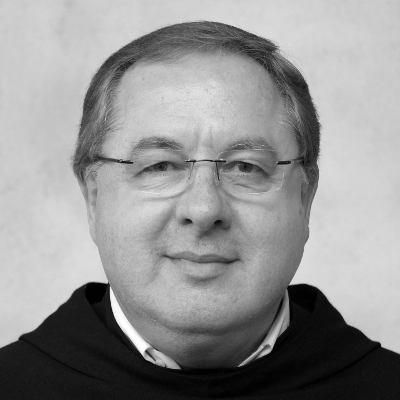
\includegraphics[width=0.29\textwidth]{immagini/enzo.jpg}
\end{wrapfigure}
\noindent Nel mese di luglio del 1997 si concludeva il Capitolo Provinciale Ordinario. L’ultimo atto fu la 
conferma dei candidati presentati dal Ministro provinciale alla guida delle varie comunità. Per 
Trieste non venne presentato alcun candidato, e il Capitolo diede il consenso perché l’elezione 
venisse fatta in seguito dal Definitorio provinciale. Non mi posi tante domande sul motivo per 
cui non fosse stato presentato un candidato per Trieste. La mia preoccupazione era di tornare a 
Roma san Marco il più presto possibile. Mi attendevano i campi estivi con i giovani della 
parrocchia. Terminato il pranzo, mi affrettai a mettere la valigia in macchina per partire. Mentre 
stavo salendo in auto il Provinciale mi chiamò e mi disse che avrebbe presentato me al 
Definitorio come guardiano e parroco di san Francesco di Trieste. Mi venne un colpo. Pensai ai 
giovani di Roma, alla gente che avevo conosciuto e amato in quella che è stata la mia prima 
esperienza pastorale. Lasciare la Città eterna per andare a Trieste mi disorientava. Eppure, prima 
o poi sarebbe accaduto. Misi davanti qualche perplessità. Tra queste che un friulano potrebbe 
non essere ben accolto dai triestini. Il Provinciale fece leva sul voto di obbedienza ed io, curioso 
e trepidante, dissi di sì.

Il 4 ottobre, festa del patrono san Francesco, iniziai il mio ministero di parroco alla presenza del 
buon vescovo Eugenio Ravignani, che presiedette la S. Messa e mi conferì il ministero di 
parroco.
%\medbreak

Memore delle parole di mia nonna che diceva: \textit{quando vai in un posto nuovo per un anno, un
mese ed un giorno taci e ascolta}, cercai di inserirmi nel cammino della Comunità parrocchiale
così come l’aveva tracciato il mio predecessore fr. Lorenzo Gottardello. In questo mi furono di 
aiuto specialmente fr. Luigi De Concini, fr. Enzo Piovesan, fr. Armando Berton, che 
conoscevano bene non solo la realtà parrocchiale, ma anche quella cittadina e diocesana.
Fu una sorpresa l’accoglienza dei triestini. Devo dire, pur con le difficoltà normali 
dell’inserimento in un nuovo contesto, di essere stato aiutato con generosità e pazienza non solo 
dai miei frati, ma anche dai collaboratori laici e da uno stile tipicamente triestino che riassumo 
nel motto: \enquote{\textit{Che la vadi ben, che la vadi mal... sempre alegri e mai passion, viva la' e po bon!}}.
Ai frati sopra citati si aggiunsero nello stesso anno fr. Bruno Garbo, e in quello successivo fr. 
Bruno Pesenti in sostituzione di fr. Enzo Piovesan. Poi arrivarono in anni differenti fr. Antonio 
Pecar, fr. Gianluigi Poirè, fr. Antonio Vitale Bommarco arcivescovo emerito di Gorizia, fr. 
Nicola Gottardo e fr. Renato Zanello. Da tutti ho avuto consiglio e sostegno nel servizio alle 
Comunità conventuale e parrocchiale e, pur con i limiti umani che ciascuno porta con sè, mi pare 
di poter dire che abbiamo dato una buona testimonianza di fraternità.
%\medbreak

Non posso dimenticare il fraterno rapporto che ha legato le due comunità religiose della nostra 
parrocchia: quella dei frati e delle suore Dimesse.
Resta in me un ricordo indelebile e pieno di gratitudine l’aiuto e la vicinanza delle suore 
impegnate non solo nella preziosa opera educativa della loro scuola, ma anche nella catechesi dei 
ragazzi, nell’animazione degli anziani e anche nel sovvenire ad alcune necessità della comunità 
dei frati. A quest’opera si devono aggiungere le catechiste e i catechisti, gli animatori e le 
animatrici, che si sono prodigati nell’offrire ai ragazzi e ai giovanissimi un cammino di crescita 
umana e cristiana, organizzando durante l’anno, oltre gli incontri settimanali, anche alcune 
iniziative straordinarie come le uscite e i campi estivi.
%\medbreak

Un ruolo importante l’hanno avuto i Consigli parrocchiali, quello pastorale e quello per gli Affari 
Economici. Ne hanno fatto parte persone coinvolte nella vita della Comunità e capaci non solo di 
consigliare, ma anche di impegnarsi direttamente nella realizzazione delle iniziative proposte. 
Ricordo come una benedizione le celebrazioni domenicali e festive, i ritiri spirituali di avvento e 
quaresima alle Beatitudini, la lectio divina settimanale, i centri di ascolto nelle famiglie, i corsi 
per fidanzati, la catechesi in preparazione al battesimo dei piccoli, o per l’iniziazione cristiana 
degli adulti, l’attenzione della Fraternitas verso gli anziani e i malati, i pellegrinaggi.
Una particolare attenzione venne data alle associazioni tipicamente francescane: Ordine 
Francescano Secolare, Gioventù Francescana e Milizia dell’Immacolata. Era mio desiderio che 
queste associazioni sviluppassero al meglio le loro potenzialità, ritenendo la loro presenza un 
dono prezioso non solo per noi frati ma anche per tutta la comunità parrocchiale. Fu una grazia 
quando venne a Trieste fr. Bruno Pesenti al quale affidai l’assistenza spirituale di OFS e MI. Lui 
ce la mise tutta e vi riuscì bene.
%\medbreak

Pur avendo avuto la fortuna di vivere a Trieste prima della crisi economica non sono mancati i 
poveri che bussavano alla porta. Gli aiuti caritas venivano gestiti dalla S. Vincenzo o 
direttamente dal parroco e da fr. Armando. C’era bisogno di una iniezione di forze nuove per un 
coinvolgimento dell’intera comunità parrocchiale. Ricordo che i primi passi di questo tentativo 
non furono facili, ma poi tutto si accomodò e si riuscì ad ottenere un buon servizio. Ricordo 
anche la generosità della comunità ad ogni mio appello per venire incontro ai nostri fratelli più 
sfortunati. Rammento un episodio per tutti. Avevo conosciuto una famiglia della parrocchia 
(papà, mamma e una figlia). I genitori erano disoccupati e non erano stati in grado per troppi 
mesi di pagare l’affitto ricevendo così lo sfratto esecutivo. Parlai con l’amministratore del 
condominio che si dimostrò comprensivo e si adoperò per trovare una soluzione con i proprietari. 
Bisognava trovare la cifra di £. 6.000.000 per fare rientrare il tutto. La domenica successiva 
raccontai ai fedeli la vicenda durante la s. Messa e come risposta ricevetti subito un assegno 
corrispondente la somma da pagare. Non fu l’unico caso in cui la Divina Provvidenza mostrò 
prontamente il suo volto.
%\medbreak

Avrei voluto rinnovare la nostra chiesa. Già la Provvidenza ci era venuta in aiuto con una 
cospicua eredità, di cui però ha beneficiato il mio successore fr. Lino, realizzando un progetto 
più ampio che ora tutti possiamo ammirare. L’unica cosa che riuscii a mettere in cantiere fu il 
battistero di cui la chiesa era sprovvista e ad inaugurarlo proprio nella mia ultima Pasqua a 
Trieste. Anche in questa occasione apprezzai la sinergia che si era creata attorno alla 
realizzazione di quest’opera. Un’opera dovuta alle continue sollecitazioni del p. Bommarco, che 
mi diceva spesso: “\textit{Se vuoi, puoi! Non bisogna attendere la Provvidenza con le mani in mano.
Tu inizia l’opera e vedrai che Lei si farà viva}”. Il denaro necessario per la realizzazione
dell’opera è arrivato da un lascito di una nostra parrocchiana il giorno stesso in cui P. Bommarco 
lasciava questo mondo. Per questo ho voluto che ci fosse una targa a ricordare l’offerente e 
l’Arcivescovo emerito di Gorizia p. Antonio Vitale. Ambedue erano stati il volto della 
Provvidenza in quell’occasione.
%\medbreak

Per me quella in san Francesco a Trieste è stata la prima esperienza come parroco. Tante cose 
potrei dire ancora, ma mi fermo qui. Ho sempre immaginato il parroco come un buon direttore 
d’orchestra, che favorisce l’accordo di tutti gli strumenti e di tutte le voci nell’esecuzione 
dell’opera di un Altro, in questo caso di Dio. Ho avuto la grazia di avere un’opera, di aver avuto 
strumenti e voci, e fratelli in grado di suonare e cantare. La mia speranza è di aver interpretato 
bene l’opera e di averla diretta al meglio delle mie possibilità rimanendo fedele a Colui che l’ha 
composta.
\begin{flushright}
\textit{fra Enzo M.}
\end{flushright}
\endgroup
\newpage
\begin{center}
\textbf{\Large p. LINO PELLANDA}\\
	\textit{parroco dal 2005 al 2013}
\end{center}
\bigbreak
\begingroup
\setlength\intextsep{0pt}
\begin{wrapfigure}[6]{l}{0.29\textwidth}
\centering
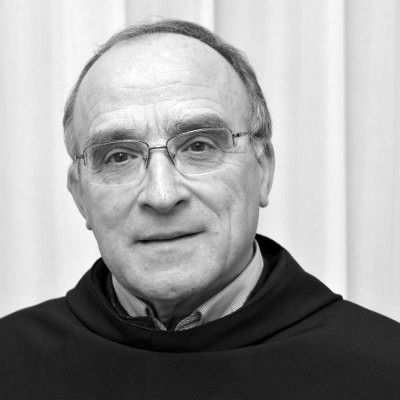
\includegraphics[width=0.29\textwidth]{immagini/lino.jpg}
\end{wrapfigure}
\noindent Il mio primo incontro con la comunità parrocchiale di S. Francesco di Trieste, risale al 
maggio 1973 quando sono stato invitato da P. Olindo con altri confratelli neo-sacerdoti a celebrare 
l'Eucaristia nel giorno di Pentecoste.
\bigbreak
\noindent \textbf{2005-2008}
\medbreak
\noindent Dopo trent'anni, il 4 ottobre 2005, sono ritornato come Parroco, accompagnato da queste 
parole di un caro amico frate: ``Auguri tanti per il nuovo ministero a Trieste. Sarà dura far seguito a 
p. Enzo, ma sono sicuro che sarai amato come lo è stato lui''.
E, davvero, ho trovato in Parrocchia un buon clima di amicizia e di collaborazione della comunità 
religiosa con i laici, per cui, valorizzando il lavoro svolto da chi mi aveva preceduto, non ho 
avvertito la necessità di “cambiare per cambiare” ma di continuare in quel cammino pastorale, 
curando sempre lo stile francescano dell'accoglienza e avendo un'attenzione particolare alla vita e 
alle linee pastorali della Diocesi che, per quell'anno, aveva scelto il tema della “famiglia”.
Era poi in corso in quei mesi nel Decanato di S. Antonio Taumaturgo (di cui fa parte la nostra 
parrocchia) e programmata per il mese di Dicembre nella nostra Parrocchia, la Visita Pastorale del 
Vescovo, Mons. E. Ravignani.
Ho avuto così l'opportunità di conoscere subito e da vicino, con gli incontri, fatti insieme, dei CPP e 
CPAE, degli operatori della catechesi, liturgia e carità, la realtà delle Parrocchie del nostro 
Decanato. Ma ciò che più mi stava a cuore, era conoscere i nuovi parrocchiani nelle loro case e, a 
mia volta, farmi conoscere.
Lo strumento tradizionalmente più adatto, anche come evangelizzazione, era la “visita e la 
benedizione delle famiglie”. Naturalmente, la realtà lavorativa e familiare rispetto a 15-20 anni 
prima era molto cambiata: in molti casi la gente rientrava dopo le 19.30; gli anziani, ad una certa 
ora avevano difficoltà ad aprire; non mancava poi una certa mobilità e la presenza negli alloggi di 
tanti studenti universitari. 
Nonostante ciò, per me e credo anche per la gente che ne ha beneficiato, è stata una bella esperienza 
bussare alla porta di tutte le famiglie e condividere con loro una parola, un'informazione sulla 
Parrocchia, un augurio, una preghiera; ed è pure stato facile accettare con “letizia francescana” 
qualche raro rifiuto all'accoglienza. Purtroppo mi è stato possibile realizzare questo impegno 
pastorale per soli due anni, a causa dei lavori di ristrutturazione della chiesa prima e del convento, 
poi.
\bigbreak
\noindent \textbf{2008-2010}
\medbreak
\noindent L'anno 2008 si è aperto con un' interessante mostra fotografica “da 70 anni FRA noi” che 
illustrava i 70 anni di presenza e di lavoro dei frati della comunità di via Giulia dal 1938: a favore 
della popolazione del quartiere fino al 1965 e poi della comunità parrocchiale di S. Francesco che, il 
20 Aprile, ha voluto celebrare solennemente l'anniversario del ritorno dei Frati Minori Conventuali 
a Trieste.
Pochi mesi dopo, alla fine del mese di luglio, sono iniziati i grandi lavori di ristrutturazione della 
chiesa: lavori urgenti e necessari a 60 anni dall'apertura al culto della chiesa.
Sembrava che dovessero partire già con la primavera-estate 2006 ma poi, per le necessarie 
autorizzazioni e approvazioni dei progetti, ci vollero ancora due anni di tempo.
Gli interventi avrebbero interessato un po' tutta la chiesa: risanamento e nuova pavimentazione della 
navata e del presbiterio che, in alcuni punti, si era sollevato di 15-20 cm; riapertura delle finestre 
delle cappelle laterali con l'apertura di nuove finestre nel presbiterio; rifacimento delle condotte del 
riscaldamento e nuova illuminazione e amplificazione; e ancora, l'adeguamento liturgico del 
presbiterio: altare, ambone, custodia eucaristica e sede del Presidente, completando così la prima 
opera di adeguamento liturgico, il nuovo fonte battesimale, realizzata nel 2005.
Prima, però, bisognava risolvere un problema logistico: come eseguire i lavori, rispettando le norme 
di sicurezza e nello stesso tempo continuare lo svolgimento delle celebrazioni liturgiche domenicali 
in chiesa, non avendo a disposizione altri locali sufficientemente grandi per accogliere i fedeli?
Con l'impegno e la disponibilità da parte di tutti: tecnici, imprese e parrocchiani si è riusciti ad 
assicurare sempre la celebrazione dell'Eucaristia domenicale occupando ora il lato destro ora il 
sinistro della navata e spostando più volte l'altare e i banchi a seconda delle esigenze dei lavori.
Ma per poter celebrare con dignità, era anche necessario pulire la chiesa: impresa non 
semplice, tenendo conto dello stato in cui era ridotta dopo una settimana di lavoro. 
Inizialmente c'era chi proponeva di affidare il lavoro di pulizia ad una cooperativa, ma poi ha vinto 
la generosità dei parrocchiani che, ogni sabato, assieme ai loro sacerdoti, si rendevano disponibili a 
pulire la chiesa per renderla così idonea per le celebrazioni.
I lavori, secondo le previsioni, avrebbero dovuto concludersi per Natale, invece 
proseguirono fino a maggio 2009 con la posa in opera del pavimento della navata e del presbiterio 
che ha permesso la celebrazione della Messa di Prima Comunione, domenica 24 maggio. 
E' seguita una lunga pausa di riflessione e confronto per trovare la soluzione migliore riguardante 
l'adeguamento liturgico del presbiterio. Alla fine, nella scelta dei vari elementi liturgici, si è deciso 
di mantenere la chiesa di S. Francesco nella sua semplicità francescana, recuperando anche alcune 
parti ed elementi presenti nel vecchio presbiterio.
E così il 17 aprile 2010 c'è stata la solenne consacrazione dell'altare con Mons. E. 
Ravignani, Vescovo emerito di Trieste, preceduta il giorno prima dalla presentazione dei lavori e 
dal concerto della Cappella Antoniana di Padova. 
Domenica 18 aprile i festeggiamenti si sono conclusi celebrando con grande gioia il 50° 
anniversario di sacerdozio di p. Olindo Baldassa e i 90 anni di p. Luigi de Concini, frati che tanto 
hanno fatto per la Parrocchia e che sono stati molto amati dai parrocchiani di S.Francesco.
\bigbreak
\needspace{3\baselineskip}
\noindent \textbf{2010-2013}
\medbreak
\noindent Conclusi i lavori in chiesa, per dare nuovo slancio alla comunità parrocchiale, era mio 
desiderio programmare una missione popolare parrocchiale, come già si stava facendo in altre 
parrocchie di Trieste, con un anno di preparazione e poi un altro per la celebrazione. 
Ma tutto rimase nel cassetto delle buone intenzioni quando mi resi conto che si trattava di una 
iniziativa pastorale molto impegnativa e, soprattutto, perché il nuovo Vescovo Mons. Giampaolo 
Crepaldi, a pochi mesi dal suo ingresso (4 ottobre 2009), aveva manifestato l'intenzione di proporre 
alla Diocesi un Sinodo Diocesano. 
E difatti, il 3 novembre 2010, nella festività di San Giusto, diede l'annuncio del Sinodo, invitando la 
Diocesi a prepararsi con due anni di intensa attività pastorale. 
Il tema del primo anno sarebbe stato “l'ascolto della Parola” e “l'Eucaristia” nel secondo; senza 
dimenticare che era iniziata anche la preparazione al Convegno ecclesiale di “Aquileia 2”.
Non è stato quindi facile seguire tutte le proposte che venivano suggerite a livello diocesano, 
decanale e parrocchiale, e integrarle nella pastorale ordinaria con la catechesi dell'iniziazione 
cristiana, la liturgia, la carità e l'ennesimo rilancio dell'Oratorio. 
Vorrei ricordare solo alcune di queste iniziative:
\begin{itemize}
	\item il rinnovato impegno per i Gruppi di ascolto della Parola nelle case, con qualche buon risultato;
	\item il tempo dedicato alla “lectio divina” sul tema dell'anno, in particolare nei venerdì di Quaresima, 
cui seguiva la “cena povera”;
	\item la proposta dei Ritiri spirituali parrocchiali all'inizio dell'Avvento e della Quaresima;
	\item i Pellegrinaggi parrocchiali a Torino per l'esposizione della S. Sindone e ad Assisi, Greccio, 
Cascia e il Pellegrinaggio della Regione FVG per l'offerta dell'olio alla Tomba di San Francesco il 4 
ottobre 2012, che mi vide molto impegnato come responsabile diocesano.
\end{itemize}
E poi, non è mai mancato l'impegno per la Caritas parrocchiale, grazie soprattutto a colui 
che per vari anni e fino a pochi mesi dalla morte ne è stato il promotore e l'animatore e che desidero 
ricordare con tanta gratitudine e affetto: Aldo Patriarca. 
Ad Aldo stavano davvero a cuore i poveri! Per anni con la Caritas li ha accolti, si è interessato a 
loro ed ha cercato di dare una risposta ai loro problemi.
Sapeva interrompere le ferie per ritornare in Parrocchia ad accoglierli nei lunedì, anche durante 
l'estate perché, diceva, “i poveri non vanno in ferie”.
Con Aldo e gli altri operatori della Caritas parrocchiale si è collaborato molto con quella diocesana, 
con i servizi sociali del Comune e con il Fondo di Solidarietà della Provincia di S. Antonio, 
coinvolgendo e sensibilizzando con varie iniziative e riflessioni tutta la comunità parrocchiale, che 
ha sempre risposto generosamente alle proposte pro – Caritas, come la tavola della carità, la 
preparazione e le offerte per l'ulivo, i mercatini della Fraternitas e le raccolte per le emergenze.
Nel  terminare queste note degli anni del mio servizio pastorale a Trieste, desidero dire un 
grazie al Signore ricordando tre confratelli, che Egli ha chiamato a sé, e che mi hanno accolto e 
introdotto, con carità e pazienza, nella comunità conventuale e parrocchiale di S. Francesco: fra 
Armando Berton, p. Luigi de Concini e p. Bruno Pesenti.
Con i loro esempi, consigli e conoscenze della Parrocchia e dei parrocchiani mi hanno aiutato a 
vivere con serenità le gioie e le fatiche pastorali negli otto anni trascorsi in una bella città come 
Trieste, assieme a tanti fratelli e sorelle che mi hanno accolto e voluto bene e che io ho cercato di 
amare e servire con la grazia del Signore e lo spirito di San Francesco. 
\begin{flushright}
\textit{p. Lino}
\end{flushright}
\endgroup
\newpage
\begin{center}
\textbf{\Large p. TIBERIO ZILIO}\\
	\textit{parroco dal 2013}
\end{center}
\bigbreak
\begingroup
\setlength\intextsep{0pt}
\begin{wrapfigure}[7]{l}{0.29\textwidth}
\centering
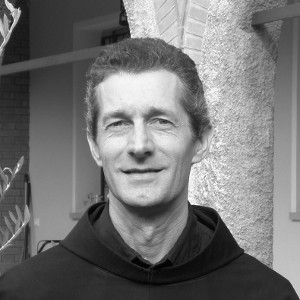
\includegraphics[width=0.29\textwidth]{immagini/tiberio.jpg}
\end{wrapfigure}
\noindent Se il valore di un parroco si misura dalle opere che ha realizzato, beh, allora anch’io posso
vantare (mio malgrado!) di aver già compiuto qualcosa in questi primi due anni: il risanamento 
della sala ``Fraternitas'' che era circondata dalle acque a causa di un inceppato (perché vetusto) 
funzionamento di drenaggio dell’intercapedine e del solaio (già qualche buon parrocchiano mi 
chiama scherzosamente ``fra Tiberio delle acque piovane''), e la metanizzazione con il rifacimento 
della centrale termica della chiesa, che è stato un vero investimento economico ed ecologico. 
Ma…devo proprio raccontare qualcosa anch’io? Allora vi parlo dei miei sogni, insieme ai miei 
attuali confratelli e parrocchiani. 

Se non è stato facile per i miei predecessori assumere e rafforzare un’eredità pastorale e 
spirituale come quella della parrocchia in questione, tanto di più per me che, nonostante i miei 48 
anni di età, sono alla mia prima esperienza di parroco. E non dite che sono avvantaggiato per il fatto 
che nei quattro anni precedenti ero già qui a Trieste come vicario parrocchiale, perché quando si 
assume il ruolo di parroco anche le relazioni cambiano. Eccome! Ho comunque sempre sentito 
l’appoggio e l’affetto di tutti, \textit{in primis} della mia fraternità conventuale, soprattutto nella buona 
persona di p. Bruno, il veterano, che dopo il suo panegirico nella celebrazione del mio insediamento 
(4 ottobre 2013) ho quasi subito avuto la grazia di accompagnarlo nella malattia. Con me, ora, 
fanno fraternità p. Antonio Renzini, p. Antonio Pastorello e p. Franco Bonafé. 

Sogni? Ideali? Scelte da fare? Strade da percorrere? Noi frati di via Giulia siamo 
perfettamente consapevoli che non dobbiamo inventare proprio niente; c’è solo da portare avanti 
quanto di buono è stato fatto (grazie a quanti ci hanno preceduto!) mantenendo in mezzo a noi Gesù 
Cristo, autore e perfezionatore della nostra fede e unità. E questo con lo stile inconfondibilmente 
francescano, caratterizzato da fraternità, minorità, letizia. E rimanere uniti al Vescovo e alla chiesa. 

Mi pare di poter dire coralmente quanto segue: la nostra priorità parrocchiale deve essere la 
formazione  cristiana, a tutti i livelli, soprattutto ora, giunti quasi al termine del Sinodo diocesano 
indetto dal nostro Arcivescovo, mons. Crepaldi (terminerà solennemente il 3 novembre prossimo).
Per formazione intendiamo: formazione di giovani animatori e valorizzazione dell’Oratorio e degli 
spazi ricreativi; mettere al centro dell’attenzione pastorale le famiglie (in particolare quelle giovani) 
sostenendole con incontri di formazione e condivisione per le coppie, di animazione per i figli, di 
inserimento nel vivo della nostra celebrazione eucaristica domenicale delle ore 10; accompagnare le 
coppie in preparazione al matrimonio (fin dal primo periodo di fidanzamento) e, dopo la 
celebrazione del matrimonio, creare momenti di condivisione e sostegno. Anche la richiesta del 
battesimo per i figli sarà per noi un’occasione di “aggancio” per accompagnare le famiglie nel 
cammino di fede dei bambini. Non potremo trascurare la crescente richiesta di formazione cristiana 
per adulti.

Un aspetto importante al giorno d'oggi è anche la comunicazione: siamo convinti della necessità di una corretta
informazione, per cui stiamo già valorizzando gli strumenti a nostra disposizione, come lo spazio nelle bacheche all'interno della chiesa, la divulgazione del foglietto domenicale ed il sito internet.

Certamente continueranno a starci a cuore la liturgia e l’attenzione per gli ultimi (e quindi 
Caritas e Fraternitas, il gruppo degli anziani), come i due movimenti fondamentali di questo 
essenziale organo umano (diastole e sistole); ma ancor più, da francescani, non potremo rinunciare 
ad accompagnare, incoraggiare e rilanciare l’Ordine Francescano Secolare e la Milizia 
dell’Immacolata: mancherebbe una parte importante della spiritualità parrocchiale guidata da frati 
francescani.

Un’ultima cosa? Sì, ed è lo spirito di fondo, l’approccio evangelico per fare autenticamente 
esperienza di chiesa, in parrocchia, e quindi crescere ed avere futuro: APERTURA, allargare il 
cerchio. In questi primi due anni da parroco ho osato (ora parlo al singolare) andare oltre al 
gruppetto di persone squisite e disponibilissime che portavano avanti praticamente tutto, con fatica 
e tanta gioia. Senza volerlo non ci si è accorti che nel corso dei decenni sono arrivate in parrocchia, 
e vivono la liturgia con noi, molte persone e famiglie nuove desiderose di inserirsi, ma timorose nel 
chiedere o esporsi. Alzare lo sguardo attorno a noi e rompere certe ingenue catene, sono gesti 
fondamentali affinché anche una semplice parrocchia come la nostra non soffochi e diventi sterile. 
Cambiare ruolo o fare un semplice passo indietro perché un altro possa mettersi nel cerchio con noi, 
non ci è facile e non è indolore: lo sanno bene ora i nostri collaboratori e corresponsabili! Ma stanno 
anche sperimentando la gioia che, insieme, è più bello. E, soprattutto, non siamo sempre gli stessi!

Grazie di cuore ai due gioielli della parrocchia (i membri del Consiglio Pastorale e quelli del 
Consiglio Economico) che sono davvero una forza entusiasmante per comunicare e testimoniare il 
Vangelo e i valori della comunità cristiana. Per sentirci chiesa nella Chiesa universale e diocesana, 
oltre alla Bibbia e alle Fonti Francescane stiamo prendendo come guida l’esortazione pastorale e 
l’enciclica di papa Francesco: \textit{Evangelii Gaudium} e \textit{Laudato Si’}. Ci sentiamo in una botte di ferro! 
\needspace{4\baselineskip}
Ci aiuterà in questo la (nuova di zecca) Commissione parrocchiale “Missione - Carità - 
Evangelizzazione”.

\noindent Il Signore vi dia pace!
\begin{flushright}
\textit{fra Tiberio}
\end{flushright}
\endgroup
\chapter{I parrocchiani raccontano}
\phantomsection
\addcontentsline{toc}{section}{Le suore Dimesse di Maria Immacolata}
\begin{center}
\textbf{\Large Le suore Dimesse di Maria Immacolata}
\end{center}
\bigbreak
\noindent \textit{Ripensando all’esperienza di Trieste…}
\medbreak
\noindent Sono arrivata a Trieste nell’ottobre 1968 per frequentare il secondo anno di Università alla
facoltà di Scienze naturali. Avevo 21 anni, ero suora professa da due anni e vivevo nella comunità 
delle suore Dimesse, allora formata da 18 sorelle. I rapporti con la comunità dei frati della 
parrocchia di San Francesco erano limitati al servizio della Celebrazione Eucaristica che p. 
Anselmo - ogni giorno (con puntualità) - ci assicurava nella nostra cappellina. La vita di studente 
però mi stava stretta; così ho chiesto ed ottenuto di iniziare ad insegnare nella nostra Scuola Media 
e di frequentare il triennio di Scienze religiose in Seminario. Sentivo anche un forte desiderio di 
lavorare in parrocchia e di collaborare come catechista. Desideravo infatti sentirmi parte viva della 
Comunità parrocchiale che avvertivo come realtà astratta. Così, pur senza alcuna esperienza, mi 
sono presentata al Parroco, p. Olindo, il quale mi accolse con molta fraternità e mi affidò subito un 
gruppo di vivaci ragazzini da preparare per la Prima Comunione. L’incontro di Catechesi seguiva la 
S. Messa domenicale, e questo facilitò senz’altro il mio compito. 

Dopo quest’inizio la collaborazione è andata via via intensificandosi e coinvolse anche le 
altre suore che trovarono sempre, da parte dei parroci e degli altri frati, fraterna accoglienza, stima e 
sostegno. Io personalmente devo molto alla comunità di San Francesco nella quale ho operato fino 
al 2000. Qui ho sperimentato il significato di Chiesa come Comunità di persone che la Fede nella 
Parola fa sentire fratelli; qui mi sono appassionata di “pastorale”… Ricordo i campiscuola con i 
ragazzi,  condivisi con p. Enzo e gli indimenticabili animatori, le giornate di ritiro della comunità 
alle Beatitudini… Ricordo l’esperienza dei centri di ascolto sulla Parola, ospitati nelle famiglie, nati 
dopo la Missione parrocchiale. Sono ricordi che mi riempiono di gratitudine e che conservo in cuore 
come doni della Bontà del Signore. San Francesco (ricordo i  ragazzi della GIFRA e il terz’ordine 
francescano) è un santo che mi ha sempre accompagnata e che, proprio ora, di ritorno da un 
campeggio speciale, vissuto ad Assisi con una trentina di ragazzi della mia attuale parrocchia, ho 
riscoperto in una novità sorprendente.
\begin{flushright}
\textit{Suor Fabrizia Baldo}
\end{flushright}
\bigskip
\phantomsection
\addcontentsline{toc}{section}{La Milizia dell'Immacolata}
\begin{center}
\textbf{\Large La Milizia dell'Immacolata}
\end{center}
\bigbreak
\noindent La Milizia dell’Immacolata è presente nella nostra Parrocchia fin dagli inizi dell’arrivo dei Frati
Minori Conventuali a Trieste, accolta e seguita quale espressione del carisma francescano e 
occasione di crescita nella vita cristiana.

Numerose note di cronaca dei frati ne tracciano, infatti, le attività e lo sviluppo.

Personalmente l’ho conosciuta attraverso mia zia Lina, devota francescana e mariana, che mi passò 
un libricino con la storia della M.I., le invocazioni e le preghiere di affidamento a Maria.

All’epoca la M.I. era seguita da p. Ruggero, poi sostituito da p. Bruno Garbo, che diedero nuova 
vitalità e ripresa partendo dal Gruppo del Rosario con nuove consacrazioni, incontri di formazione 
mariana e kolbiana ed altre iniziative ed incontri divulgativi, anche attraverso alcune conferenze di 
p. Terenzio De Poi, delegato provinciale M.I., e alcuni viaggi a Padova per dei Convegni Mariani.

Il mio coinvolgimento più spirituale, però, nacque in seguito all’anno Giubilare 2000 quando p. 
Bruno Pesenti, nuovo assistente della M.I., quale frutto della celebrazione Giubilare avviò un corso 
di formazione M.I. che l’8 dicembre 2001 mi portò, con altri 10 militi, alla consacrazione.

In questi anni il nostro gruppo è cresciuto sia numericamente, anche con militi provenienti da fuori 
provincia, che nella partecipazione diretta alle attività M.I. a livello regionale, dove personalmente 
ho svolto il ruolo di consigliere ed economo.

Abbiamo partecipato anche a convegni e consigli a livello nazionale, infatti la M.I. è una 
Associazione Mariana approvata dal Pontificio Consiglio per i laici con propri statuti e consigli a 
livello locale, regionale e nazionale.

Dal 2002 abbiamo il nostro Consiglio Locale, con attuale assistente il p. Antonio Pastorello, che 
organizza le attività di catechesi, di collaborazione con il Consiglio Regionale e di servizio in 
parrocchia.

Siamo una ventina di militi e siamo impegnati nell’animazione del Rosario e delle adorazioni 
eucaristiche, nelle letture alle S. Messe, nella cura degli addobbi floreali, nella raccolta di offerte 
per le adozioni a distanza.

Personalmente questa partecipazione e catechesi ha contribuito molto alla mia formazione cristiana 
in una forma nuova con l’Immacolata, nostra mediatrice presso Dio.
\begin{flushright}
\textit{Claudio Otti}
\end{flushright}
\bigskip
\phantomsection
\addcontentsline{toc}{section}{L'Ordine Francescano Secolare}
\begin{center}
\textbf{\Large L'Ordine Francescano Secolare}
\end{center}
\bigbreak
\noindent Nel gennaio del 1939 il Padre Superiore riceve l'autorizzazione del Vescovo di erigere la fraternità 
dell'Ordine Francescano Secolare (allora Terz’Ordine Francescano). Comincia la vita della nostra 
fraternità, intitolata a San Francesco d'Assisi. 
Secondo l'uso del tempo, la fraternità vanta una sezione femminile e  una sezione maschile, che si 
è esaurita presto. 

Le terziarie si incontravano una volta al mese (domenica). Erano tuttavia impegnate in servizi 
diversificati: pulizia della chiesa, cura degli arredi sacri e dell'altare, cura assidua del guardaroba 
dei frati; catechesi ai bambini per la Prima Comunione e per la Cresima. 

Grande attenzione veniva prestata ai poveri. Una nostra sorella confezionava e offriva le 
vesticciole bianche per i battesimi. 

Un buon gruppo di terziarie erano "delegate" per le missioni e ogni mese raccoglievano denaro e 
materiale (vesti-viveri-medicinali) da inviare in zone missionarie. Troviamo la nostra fraternità 
impegnata a raccogliere porta a porta - ogni mese - offerte in denaro per costruire la chiesa di San 
Francesco, sorta nel tempo, in Via Giulia. Così per lunghi anni. Fa storia l'agnello pasquale offerto 
ai frati per la mensa di Pasqua. 

Piano piano le terziarie muoiono senza grande ricambio generazionale. Solo all'inizio degli anni '90 
la fraternità si "ripopola". 

Oggi siamo una piccola fraternità che cerca di rifiorire, sia dal punto di vista numerico che come 
attività in parrocchia e fuori. 

C'è partecipazione attiva ai ritiri diocesani e agli incontri proposti dal centro regionale. 

Negli anni abbiamo cercato di essere presenti  nel Consiglio Pastorale, nella catechesi ai bambini, 
ai giovani ed adulti, e nella preparazione di coppie per il matrimonio. 

Una nostra sorella è presente nell'animazione degli anziani assistiti dalla Fraternitas. 

Nell'ambito della carità, da lungo tempo condividiamo il servizio alla mensa dei poveri allestita 
presso il convento dei PP. Cappuccini, a Montuzza. Inoltre come fraternità portiamo avanti 
un'adozione a distanza in Romania tramite il centro missionario O.F.S..

Negli anni abbiamo cercato di creare un buon rapporto con i frati presenti nella nostra parrocchia 
valorizzando in particolare due momenti: il rinnovo delle nostre professioni il 29 novembre, cui 
segue una cena e l'estrazione dei santi protettori il 6 gennaio, assieme alla Milizia dell'Immacolata. 

Siamo grati a tutti i frati che ci hanno dato assistenza perché da ognuno abbiamo potuto imparare 
qualcosa, ma non possiamo non ricordare in modo particolare, anche se con un po' di rimpianto, 
P. Bruno Pesenti che ci ha lasciato troppo presto. 

Il nostro auspicio, nel festeggiare questi 50 anni di vita della parrocchia, è che i fratelli e sorelle 
dell'Ordine Francescano Secolare possano essere sempre più "luce e sale" di questa comunità, 
nonostante i loro limiti e impegni che spesso li portano altrove.

\begin{flushright}
\textit{Fraternità OFS}
\end{flushright}
\bigskip
\phantomsection
\addcontentsline{toc}{section}{San Francesco, 1965-1990}
\begin{center}
\needspace{3\baselineskip}
\textbf{\Large San Francesco, 1965-1990}
\end{center}
\bigbreak
\noindent \textit{Per questo periodo ci è stato difficile reperire grandi testimonianze, poiché non sono tanti i
parrocchiani vivi e ancora presenti in parrocchia che ci possono aiutare a ricostruire la vita 
parrocchiale. Ci dispiace soprattutto là dove manca anche il racconto del parroco, mentre altrove siamo riusciti a tamponare in qualche modo. Certamente 
scartabellando tra bollettini e cronache avremmo trovato materiale interessante, ma non rientra 
nell’interesse di questo libricino. Grazie, allora, alle seguenti testimonianze:}
\medbreak
\noindent ``P. Olindo è stato il parroco della mia infanzia, e con lui ho ricevuto la Prima Comunione 
(nel 1974). Eravamo in tanti, quel giorno! Ricordo il Franciscanum pieno di bambini, tutti schierati 
per la foto di rito sui gradini e lui là, in mezzo, sorridente, sereno e tranquillo.
Non eravamo certo dei santi, ma non l’ho mai sentito alzare la voce.
Mi piacevano i suoi modi gentili e accoglienti, che hanno contribuito a far sì che “San Francesco” 
diventasse la “mia” parrocchia.
Ricordo il dispiacere che ho provato alla notizia del suo avvicendamento, incapace (allora come 
ora) di capirne il perché''.\par
\hfill\textit{Annamaria Berti}
\begin{center}
	\noindent\rule{0.5\textwidth}{0.4pt}
\end{center}
“In p. Olindo ho sempre visto la serena fermezza del cristiano che ha posto nella fede il 
fondamento della sua esistenza. La vocazione francescana, assolutamente coerente alle doti del suo 
carattere, ha certo illuminato tutti i suoi atteggiamenti e il suo rapporto con i parrocchiani. Mai 
impaziente, sempre disponibile, ci ha sempre donato il suo sorriso, che non era mai formale, ma 
nasceva dall’intimo, come la perfetta letizia dei Fioretti di san Francesco.
Grazie di tutto, carissimo p. Olindo! 
\medbreak
P. Germano, invece, era una persona di carattere riservato, serio e meditativo. Ho sempre 
pensato – e la realtà lo ha confermato – che avesse dei problemi, soprattutto legati alla condizione 
fisica, di cui, per una sorta di timidezza e pudore, non voleva far trasparire nulla.
\needspace{3\baselineskip}
Le sue omelie rivelavano, però, come fosse profonda la sorgente della sua fede: egli ci offriva, oltre al commento 
delle letture, il frutto delle sue personali meditazioni, che approfondivano ogni tema ed ogni spunto.
Di questo lo ringraziamo!”\par
\hfill\textit{Maria Grazia Rozzo}
\begin{center}
	\noindent\rule{0.5\textwidth}{0.4pt}
\end{center}
Sono arrivato in questa parrocchia a fine 1987, precisamente il giorno dell’Immacolata, l’8 
dicembre, dopo un week end di fatiche per il trasloco (autogestito) nella nostra nuova casa.

Abbiamo incominciato da subito a frequentare la parrocchia, prima eravamo aggregati a quella di 
via del Ronco, ed avendo due bambini piccoli, il primo in età scolare, ci siamo attivati per iniziare il 
catechismo in preparazione alla Prima Comunione. 

Ho così conosciuto il parroco p. Germano, che ci ha fraternamente accolti per inserire Daniele nel 
gruppo del primo anno.

Padre Germano purtroppo è stato poco con noi, perché in una delle prime riunioni con le famiglie 
del catechismo ci informò della sua grave malattia e del ricovero in ospedale. Di lui ricordo la 
grande serenità nel comunicarcelo e l’affidamento alla Provvidenza per quanto riguardava il 
necessario intervento, sentimenti di serenità ed affidamento che ritrovai in lui anche in clinica e che 
ho ritrovato tanti anni dopo in p. Bruno Pesenti, durante il suo ricovero e la successiva 
convalescenza, segni entrambi di insegnamento francescano e cristiano.

Ricordo anche la mia prima veglia pasquale in Parrocchia, perché molto meno partecipata di quelle 
che seguirono, forse a causa della malattia e conseguente assenza del parroco.

Nello stesso periodo ho incontrato anche p. Giambattista Bontempi, che seguiva l’oratorio ed i 
bambini del catechismo, e con lui ho iniziato a partecipare più attivamente alle attività della 
parrocchia, in particolare mi coinvolse nel servizio delle letture e nella ricerca di finanziamenti 
pubblici per l’oratorio.

Poi con l’arrivo del nuovo parroco, p. Lorenzo, il mio impegno è cresciuto non solo nel servizio 
delle letture, dove lui organizzò uno specifico corso di lettore, ma anche nella gestione economale 
della parrocchia, attraverso il nuovo CPAE al quale mi chiese di partecipare.

Fu per me un’attività nuova e molto interessante, perché ebbi modo di conoscere le varie voci di 
spesa e di entrata gestionale di una realtà parrocchiale.
Una volta acquisita padronanza nei vari conti di E/U, con l’approvazione di p. Lorenzo mi fu poi 
possibile trasferire i grandi libroni cartacei nel computer, nel frattempo acquisito, con il quale 
risultò più semplice, sicuro (senza fare le somme a mano!) e veloce gestire la contabilità 
parrocchiale.

Ci fu un’altra attività, molto significativa dal punto di vista pastorale, che nacque in quel periodo 
con p. Lorenzo: dal gennaio ‘93 venne avviato il Giornalino Parrocchiale \textit{“Due o più”} con uscita 
trimestrale, grazie all’impegno di Giovanni Masci, anche lui membro del CPAE, con cui ebbi modo 
di collaborare nella stesura grafica, sia a mezzo computer che nel Centro Stampa, allora molto 
semplice con una sola macchina ciclostyle.

Venne distribuito in parrocchia per diversi anni (fino al 1998), poi sostituito dal foglietto 
domenicale, per dare più immediatezza e sintesi alle notizie di vita parrocchiale.

Furono anni molti intensi e gioiosi, per la possibilità di partecipare, in un modo per me nuovo e più 
forte, alle attività parrocchiali, servizio poi continuato anche con i parroci che sono seguiti.

A loro il mio grazie per avere coinvolto forze nuove, come ora sta facendo anche p. Tiberio.\par
\hfill\textit{Claudio Otti}
\begin{center}
	\noindent\rule{0.5\textwidth}{0.4pt}
\end{center}
Negli scorsi decenni più volte abbiamo salutato e accolto un nuovo padre guardiano, un  
superiore, un nuovo pastore che viene a guidare la nostra parrocchia, però non ci siamo mai abituati 
a questi cambiamenti “normali” nelle parrocchie affidate a istituti religiosi e ogni volta che ne arriva 
uno nuovo è quasi un’emozione: è come una nuova fase della nostra storia, della nostra vita che 
ormai condividiamo nell’ambito della nostra comunità che ci ospita e accoglie le nostre famiglie dal 
battesimo alla fine dei nostri giorni, come un legame diretto con il Signore, con il suo Vangelo che 
esploriamo ogni domenica nel rito liturgico. Nel 1976 dopo p. Olindo Baldassa, arriva a Trieste da 
Verona,  come guardiano e parroco, il p. Innocenzo Bordin. 

Il 1976, storicamente, è l’anno del terremoto nel Friuli, della sciagura di Seveso, della  
sanguinosa guerra in Libano e dei desaparecidos in Argentina. Nell’ambito ecclesiale dopo il 
Concilio è offerto ai laici un più largo accesso a incarichi ecclesiali, anche liturgici. Parallela a 
questa accresciuta partecipazione laicale alla vita della Chiesa, si registra in seno al laicato cattolico 
una forte crisi dell'associazionismo tradizionale, cui fa riscontro una vasta fioritura internazionale di 
nuovi gruppi di spiritualità di varia natura: comunità dì base, gruppi biblici, fraternità, movimento 
carismatico, ecc., le cui attività la Chiesa tende a regolare e contenere, opponendosi a quelle 
tendenze centrifughe che non riconoscano nel vescovo un punto di riferimento.

P. Innocenzo al suo arrivo conquista  subito tutti con la sua affabilità,  la  sua capacità di  
comunicazione e il suo modo di impostare il linguaggio biblico come base per la vita quotidiana del 
cristiano. E’ sempre presente agli incontri di preparazione dei catechisti parrocchiali, molto 
numerosi sotto la sua guida.  Un’importante iniziativa è l’apertura di un ciclo di conversazioni 
sull’Antico e Nuovo Testamento che vengono seguite da un folto gruppo di ascoltatori, non solo 
parrocchiani. Anche il settimanale diocesano “Vita Nuova” ospita  le sue lezioni esegetiche sul 
Vangelo della domenica. 

Forte di una sua esperienza sulla spiritualità del cammino neocatecumenale di Kiko 
Argüello, dopo  un certo tempo accoglie anche in parrocchia la “catechesi” della stessa spiritualità, 
costituendo quindi una prima “comunità”, cui seguono anche altre successive (cinque). 

“Egli – scrive a questo proposito Bianca Maraspin – era convinto che il Cammino 
Neocatecumenale fosse uno strumento di evangelizzazione soprattutto per chi si era allontanato 
dalla Chiesa. Ad ogni inizio anno preparava i suoi catechisti con una settimana di formazione in 
montagna, e ogni mese voleva verificare come andavano le cose. Era un assiduo confessore, amato 
e ricercato perché faceva capire l’amore che Dio ha per i peccatori e che nessuno è escluso dalla sua 
misericordia”.

È di questo periodo l'uscita di un giornalino periodico dal titolo ``Il Punto'' che si occupava della vita parrocchiale
vista da varie angolature (anche se durerà solo per pochi anni: dal 1977 al 1980).

Tra le altre iniziative, da segnalare, nel 1978, l’inizio dell’attività di un gruppo di spiritualità 
familiare costituito da genitori di bambini in preparazione ai Sacramenti dell’iniziazione cristiana; 
un gruppo iniziato personalmente e poi affidato al p. Aldo Frigo. 

Di grande significato, durante la sua permanenza a Trieste, è stata la sua testimonianza di 
fede nell’affrontare momenti difficili e dolorosi della sua vita personale che hanno richiesto due 
ricoveri presso l’Ospedale Maggiore di Trieste per due interventi chirurgici (il secondo dei quali 
motivato da una grave malattia).  Anche dopo il suo trasferimento a Verona  a molti di noi è stata 
data la possibilità di continuare a seguire il suo percorso di fede anche durante la malattia terminale, 
fino al momento del “passaggio” più importante del nostro itinerario cristiano. Una testimonianza  
rimasta incancellabile nel nostro ricordo.
\begin{flushright}
\textit{Bianca Maraspin e Luigi Favotti}
\end{flushright}
\bigskip
\phantomsection
\addcontentsline{toc}{section}{San Francesco, 1990-2015}
\begin{center}
\needspace{3\baselineskip}
\textbf{\Large San Francesco, 1990-2015}
\end{center}
\bigbreak
\noindent Ad un gruppo di noi parrocchiani è stato chiesto di “raccontare” il nostro vissuto nella
comunità; lo facciamo volentieri partendo dal nostro primo approccio.
Questa non vuole essere una cronistoria di persone, fatti ed avvenimenti succedutisi in questo 
quarto di secolo e men che meno un qualcosa di letterario od impegnato, ma semplicemente  la 
testimonianza di quanto abbiamo ricevuto in questi 25 anni di vita comunitaria dai vari parroci che 
si sono succeduti, dai loro confratelli, dalle “sorelle” Dimesse alle quali siamo molto legati, dalla 
comunità tutta. In sintesi è la testimonianza di quanto sia bello, importante, gioioso sentirsi parte di 
una comunità che si ama “come Gesù ci ha amato”.

Ci rendiamo anche conto di quanti frati, laici impegnati nella parrocchia, avvenimenti non 
riusciremo a citare anche se sono e saranno sempre presenti nei nostri cuori. Sin d’ora ci scusiamo.
L’inizio di tale esperienza è personale (anche se coincidente con gli altri estensori). Tutto il resto è 
condiviso e scritto, potremmo dire, a sei mani.

Una sera, rientrando a casa dal lavoro, mia moglie Grazia mi avverte che ha chiamato al 
telefono un parrocchiano, a me ancora sconosciuto (diventato poi il mio più caro amico e troppo 
presto scomparso!!) per parlare con me. Avendo lasciato il suo numero di telefono, per pura 
cortesia, lo richiamo. Ma…probabilmente, quando di mezzo c’è lo Spirito Santo, la fatalità, la pura 
cortesia, la coincidenza non c’entrano; esiste un’altra cosa con un nome preciso: CHIAMATA.
In breve mi avvertiva che il parroco, venuto da poco a sostituire padre Germano, avrebbe avuto 
piacere di scambiare quattro chiacchiere con alcuni parrocchiani. Le “quattro” chiacchiere 
divennero ben presto impegno gioioso.

Era l’anno della “missione al popolo” (1989) e così ci propose di formare un gruppo d’ascolto 
“itinerante” nelle varie abitazioni, per approfondire le pagine della bibbia scelte di volta in volta da 
noi. Nel contempo ci chiedeva, con molta discrezione, se eravamo disposti ad un impegno più 
concreto in parrocchia.

Molti di noi (tra cui gli scriventi) risposero di sì con entusiasmo e spirito di servizio e così iniziò 
un’avventura di impegno, di fede, di comunità e soprattutto di amicizia, con Gesù Cristo al centro, 
che dura ancora.

P. Lorenzo Gottardello aveva formato attorno a sè un gruppetto di persone con lo scopo di 
programmare le attività dell’anno liturgico per rendere le celebrazioni più gioiose e partecipate. 
Ognuno di noi, avendo idee e sensibilità diverse, esprimeva in libertà il proprio pensiero nel 
preparare le varie celebrazioni. Le idee a volte erano contrapposte; p. Lorenzo ascoltava, prendeva 
nota e… con grande abilità, umiltà e pazienza, riusciva sempre a costruire un qualcosa di bello in 
cui ognuno di noi poteva riconoscersi. E’ anche così che il nostro impegno aumentava, la nostra 
amicizia cresceva e con essa cresceva anche un primo nucleo coeso su cui costruire la comunità. 
Ricordo le prime funzioni “extra messa” nei momenti forti dell’anno liturgico: “siamo in 12 … in 
13… festeggiamo i primi 15!” Scoramento? No, maggiore impegno!
Il cruccio di quel periodo (uno dei tanti) era quello di non riuscire ad avviare l’oratorio.

Un avvenimento di quel periodo è stata l’ordinazione 
sacerdotale di p. Enzo Piovesan nella nostra chiesa. E’ rimasto con noi alcuni anni e quando ha 
assunto nuovi incarichi lontano da Trieste non ha dimenticato la comunità ma, quando ha potuto ed 
ancora può, torna sempre a farci visita considerando questa parrocchia la sua casa e la sua famiglia, 
sentimenti da noi pienamente condivisi.

Molto attivo ed apprezzato, già in quel periodo, l’impegno discreto ma molto concreto delle 
suore Dimesse, che si sono sempre sentite parte attiva della nostra parrocchia.
Il tempo passava e la comunità parrocchiale cresceva. Ricordiamo, essendo impegnati in prima 
persona, la stesura del primo regolamento del CPP (Consiglio Pastorale Parrocchiale), le prime 
elezioni, i primi incontri “ufficiali”. 
Di quel periodo non si possono non ricordare due frati che per tanti di noi erano dei fratelli maggiori 
e, per i giovani, dei nonni; p. Tarcisio Lupieri e p. Luigi De Concini. La loro semplicità, bonarietà, 
spontaneità riuscivano a contagiare quanti li conoscevano.

Il tempo però correva in fretta ed un giorno (erano passati 8 anni) p. Lorenzo ci comunica 
che con il prossimo 4 ottobre (1997) ci avrebbe lasciato, avendo concluso il suo mandato.
Avevamo “sentito” dire che poteva venire a sostituirlo un Padre avanti con l’età e con poche 
motivazioni. Con fatica avevamo appena gettato le fondamenta su cui costruire una bella e solida 
comunità e, ai nostri occhi, ciò veniva messo in serio pericolo. Ai nostri occhi però, non a quelli 
dello Spirito (di questo ne siamo certi) che aveva deciso che il nostro impegno meritava sorte 
migliore. Così lo Spirito, aiutato (così pare) dalla paziente opera di convincimento del nostro p. 
Lorenzo prima e durante le elezioni a Padova, decise che era il momento di dare una bella spinta 
alla nostra comunità per collocarla su più alte cime. E chi, meglio di un ex alpino poteva riuscire 
nell’impresa se non p. Enzo Poiana? Anni meravigliosi anche se, per lui almeno il primo, non è 
stato certamente tale.

Quando sei abituato per anni ad un certo modo di rapportarti con il padre parroco, quando dai per 
scontato che ciò che è stato fatto sia inamovibile, non discutibile, e soprattutto cerchi di imporre al 
nuovo tale dei cliché, è ovvio che all’inizio ci sia malessere, scontro, incomprensione. Sta alle due 
parti, se intelligenti, trovare il punto d’incontro. Come già detto, a nostro modesto parere, le parti in 
causa erano non due ma tre; in una comunità di credenti è sempre la “terza Persona”, lo Spirito, che 
deve avere l’ultima parola! E così è stato.
La simpatia, l’esuberanza giovanile, la giovialità unita però alla gran fede che emanava nei suoi 
gesti ed azioni (ovviamente parliamo di p. Enzo) conquistarono in breve tempo non solo lo “zoccolo 
duro” dei fedeli ma attirò anche molti giovani ed adolescenti che si ritrovavano in quel linguaggio 
semplice e diretto, ancorché profondo. In quel periodo cominciarono a frequentare la nostra 
parrocchia anche fedeli di altri rioni attratti proprio da quanto sopradetto.

Nell'anno pastorale 1998/99 il giornalino trimestrale ``Due o più'' viene sostituito dal foglio 
settimanale ``Camminare insieme'', offrendo così un'informazione più immediata che continua ancora 
oggi.

Nel 2003 ha avuto inizio una bella iniziativa che continua ancora oggi e, speriamo, prosegua 
sempre: l’adorazione eucaristica per la pace ogni 13 del mese. Il Santissimo sacramento viene 
esposto dalla mattina alla sera per permettere a tutti un momento di preghiera spontanea e personale 
con il nostro Signore Gesù Cristo.  

Indimenticabili i pellegrinaggi fatti assieme a lui e, degno di nota, la partecipazione ad un incontro, 
al ``Divino Amore'' a Roma, organizzato dalla Conferenza Italiana dei Superiori Maggiori (CISM), 
con la partecipazione dei laici. L’aver portato un gruppo numeroso di parrocchiani fu motivo di 
“bonaria invidia” da parte degli altri religiosi presenti ed una bella testimonianza di vitalità della 
nostra comunità e, per gli scriventi (che erano lì presenti), momenti di grande arricchimento 
spirituale.

In quel periodo avemmo la fortuna ed il privilegio d’avere con noi p. Antonio Vitale Bommarco 
(Vescovo emerito di Gorizia) il quale aveva scelto Trieste e, perché no, p. Enzo come sua ultima 
dimora e ultimo guardiano. E’ di quel periodo la realizzazione del nuovo e bel battistero della nostra 
chiesa.

La comunità cresceva, le attività si moltiplicavano e si consolidavano attorno a p. Enzo, sempre 
pronto a sostenerci nei momenti difficili.

Oltre a p. Enzo corre l’obbligo sottolineare che in quel periodo venne ad arricchire la nostra 
comunità un frate, recentemente scomparso alla nostra vista ma indelebile nei nostri cuori: p. Bruno 
Pesenti. Bergamasco schivo, poco ciarliero ma di una profondità, fede ed umanità dono esclusivo 
dello Spirito. Noi che raccontiamo, avendo avuto momenti di “fatica fisica” in questi ultimi anni, 
possiamo testimoniare quanto coraggio, quanta certezza nel sentire il sostegno che p. Bruno riusciva 
a trasmetterci. Il più delle volte bastava un gesto, una stretta di mano, un abbraccio e ti sentivi 
pervadere d’amore. Grazie p. Bruno! 
Gli anni passano e la comunità ecclesiale si consolida; la chiesa invece, intesa come edificio fisico, 
comincia a deteriorarsi.

Il mandato di p. Enzo intanto si conclude anticipatamente; alla Basilica del Santo serve un nuovo 
Rettore, e per i suoi superiori Enzo è la persona giusta.

Lo abbiamo accompagnato in tanti al suo primo appuntamento in quel di Padova, contenti per il suo 
nuovo incarico, tristi per avere perso una guida spirituale di spessore, un ottimo parroco, un 
eccellente amico. L’unico rammarico (ovviamente scherzoso, riportando la pura cronaca di quel 
giorno) fu che la Curia Romana non diede seguito alle richieste  (per loro sacrosante) del folto 
gruppo di giovani ed adolescenti che l’accompagnava e che stava scritto su un grande telo tenuto 
ben in vista in Basilica: “P. Enzo papa subito” (o almeno santo). Ad oggi è una richiesta rimasta 
inevasa però, come suol dire proprio p. Enzo, non porre mai limiti alla Provvidenza. 

A proposito di Provvidenza: come sopradetto, la chiesa era disastrata, con l’altare maggiore 
che stava alzandosi, crepe sui gradini e tante altre cose da sistemare. Ci voleva, a sostituire p. Enzo, 
un frate “architetto” od almeno “capomastro” in grado di sobbarcarsi tale incombenza.
Chi meglio di uno che aveva sovrainteso alla ristrutturazione della chiesa a Rovereto? P. Lino 
Pellanda.

Più anziano di Enzo ma non meno dinamico, gioviale e simpatico anche se, per alcuni, sembrava un 
tantino cocciuto ed autoritario. Noi possiamo testimoniare il contrario (od anche il contrario del 
contrario?).

Il primo anno (2005-2006), con l’esperienza accumulata in tanti anni di impegno parrocchiale, li 
trascorse senza apportare modifiche allo “schema” ereditato, cercando di conoscere a fondo tutti i 
componenti della comunità, partendo da quelli più impegnati nei vari incarichi parrocchiali.
Non si occupava solo di marmi e cemento, ma la sua prima preoccupazione (divenuto piccolo 
cruccio per non averla portata a termine) fu quella di fare visita a tutte le famiglie e persone della 
nostra parrocchia, per conoscerle personalmente e portare loro la benedizione cristiana. I tanti 
impegni e la scarsità di frati non permisero di dare continuità all’opera.

Durante il suo mandato ci lasciarono fra Armando e p. Luigi (entrambi nel 2012). Li 
abbiamo accompagnati verso le case di cura (rispettivamente a Pedavena, BL, e a s. Pietro di 
Barbozza, TV) e poi verso l’ultima dimora (cimitero di Camposampiero, PD). Hanno vissuto la loro vita consacrata nel vero spirito 
francescano di povertà, obbedienza e testimonianza gioiosa di Cristo, riuscendo a trasmettere a 
quanti li hanno conosciuti questi semplici e genuini valori cristiani: Grazie!
Da segnalare che, durante i lavori di restauro all’interno della chiesa, si poneva un grosso 
interrogativo: dove officiare le varie celebrazioni, vista l’estensione in termini di tempo e superficie 
interessata da tali lavori? E’ stato, potremmo dire, un anno di “chiesa itinerante”. Con l’impegno ed 
il sacrificio di tanti parrocchiani, man mano che i lavori interessavano parte della chiesa, altare, 
banchi e tutto il necessario veniva spostato nella parte libera o già finita. 
Piccolo particolare: durante la settimana i lavori continuavano! Calcinacci, polvere e quant’altro si 
accumulavano; la buona volontà di molti riusciva, lavorando sodo di sabato (o alla vigilia delle 
celebrazioni infrasettimanali), a restituire ai fedeli una chiesa pulita e, per quanto possibile, 
praticabile. E’ stato un esempio, dei tanti, di quanto possa fare una comunità che sente la Chiesa 
come “casa propria”.

Anche con p. Lino abbiamo avuto modo di effettuare alcuni pellegrinaggi, il più importante 
ed emozionante a Torino, per l’ostensione della Sacra Sindone. Sono stati momenti importanti, oltre 
che formativi, per consolidare amicizie e stringerne di nuove con la gioia di sentirci parte attiva 
della grande famiglia che è la Chiesa. 
La soddisfazione di p. Lino è stata quella di vedere conclusa la parte più importante della 
ristrutturazione della chiesa (2009), e poi anche quella del convento (2012).

Sempre a proposito di Provvidenza (quella con la P maiuscola): nel momento in cui la 
comunità dei nostri frati era ridotta all’osso (p. Lino, p. Bruno e p. Luigi) ecco arrivare, non 
certamente per caso, un giovane frate ad arricchire la comunità: p. Tiberio Zilio (di cui diremo in 
seguito).

Il tempo scorre inesorabile ed anche per p. Lino arriva il momento del commiato (2013) alla volta 
dei Frari, a Venezia, accompagnato da tanti parrocchiani a lui grati per quanto era riuscito a 
costruire materialmente e, soprattutto, spiritualmente nella nostra comunità. 

Dunque, in questi 25 anni di rapido exursus, abbiamo avuto, a guidare il nostro “piccolo 
gregge” di san Francesco:
\begin{itemize}
	\item Un parroco umile, paziente di grande umanità e fede: p. Lorenzo;
	\item Un parroco giovane, esuberante e di grande carisma: \\p. Enzo;
	\item \sloppy Un parroco ``carro armato'' ma buono interiormente, spontaneo e di fede semplice e genuina: p. Lino.
\end{itemize}
Mancava, senza nulla togliere ai predecessori, un parroco che riassumesse, pur se in maniera 
diversa e personale, le doti dei predecessori aggiungendone un’altra tutt’altro che trascurabile per 
un francescano: rendere visibile, con il suo comportamento, il suo vivere e il suo approcciarsi alla 
comunità, il messaggio fondamentale di Francesco, l’umiltà e l’amore per Gesù Cristo senza “se” e 
senza “ma”.
“Le vie del Signore sono infinite” recita un detto. Di ciò noi possiamo portare testimonianza diretta: 
p. Tiberio, attuale guardiano e parroco. La storia, ovviamente, continua!
Starà ai giovani di oggi (che speriamo siano sempre più numerosi) raccontare i prossimi 25, 
50 e più anni di vita della nostra parrocchia. Ai “pastori” che guidano ora la parrocchia, p. Tiberio, 
p. Antonio Pastorello, p. Franco Bonafé, p. Antonio Renzini, auguriamo buon lavoro.
Comunque, se il buon giorno si vede dal mattino, siamo certi che i capitoli che seguiranno 
racconteranno “in scienza e coscienza” la grazia dello stare insieme animati e sostenuti nelle varie 
attività dalla loro presenza discreta ed illuminata.
%\medbreak

\begin{samepage}
BUON LAVORO e…. sia lodato GESU’ CRISTO! come si diceva una volta e, grazie a Dio, 
almeno nella nostra parrocchia, si è tornati a dire.
\begin{flushright}
\textit{Mario Fragiacomo, Mariuccia Del Piero, Luciana Verona}
\end{flushright}
\end{samepage}
%=========================================

\tableofcontents
\newpage
\cleartoleftpage
\thispagestyle{empty}
\null
\vfill
\noindent \small A cura della segreteria del CPP (Susanna Bologna, Gianfranco Liut e fra Tiberio).
Un grazie particolare a d. Giorgio Petrarcheni (cancelliere vescovile) e a p. Federico Santolin (segretario provinciale) per aver fornito i documenti e le foto. Foto della copertina realizzata da Marisa Pianigiani. Libro impaginato da Flavio Barisi utilizzando 
il software open-source \LaTeX.
\bigbreak
\begin{center}
settembre 2015
\end{center}
\end{document}
